\documentclass[8pt]{beamer}

\usepackage[utf8]{inputenc}
\usepackage[T1]{fontenc}

\usepackage{longtable}
\usepackage{booktabs}

\usepackage{graphicx}
\usepackage{subfig}
\usepackage{floatrow}

\usepackage{tikz}
\usetikzlibrary{arrows}

\usepackage{standalone}

\usepackage{amssymb}
\usepackage{amsmath}
\usepackage{mathrsfs}
\usepackage{mathtools}
\usepackage{dsfont}
\usepackage{bbold}
\usepackage{breqn}


\usepackage{pdfpages}
\usepackage{hyperref}

\usepackage{color}


\usetheme{ign}

\title{Traitements avancés des images de Télédétection}
\subtitle{SVM et Sélection d'attribut}
\author{Oussama ENNAFII}
\institute{ENSG}
\date{\today}

\begin{document}

	\begin{frame}[plain]
		\titlepage{}
	\end{frame}

	\section{Introduction}

	\begin{frame}{Rappel: Classification supervisée}
		\begin{figure}[H]
			\begin{center}
				\includestandalone[mode=buildnew, height=.4\textheight]{scatter_gender_dataset}
				\caption*{\tiny Exemple de problème de classification: $2$ attributs et $2$ classes.}
			\end{center}
		\end{figure}
		\begin{itemize}
			\item <1-> On observe $n$ échantillons: $\big((X^i, Y^i)\big)_{i=1,\dots,n}$
			\item <2-> Connaissant une instance $X^j = \begin{pmatrix}
			X_1^j\\
			\vdots \\
			X_d^j
			\end{pmatrix}$, il faut prédire sa classe $Y^j$ et la probabilité de cette classe.
		\end{itemize}
	\end{frame}

	\begin{frame}{Supervisé vs Non-Supervisée}
		\begin{figure}[H]
			\begin{center}
				\includestandalone[mode=buildnew, height=.4\textheight]{scatter_circles}
				\caption*{\tiny Exemple de problème de classification non supervisée: Pas de classes mais une structure se dégage.}
			\end{center}
		\end{figure}
		\begin{itemize}
			\item <1-> On observe ${(X^i)}_{i=1,\dots,n}$ sans les classes $\longrightarrow$ non supervisée,
			\item <2-> On observe ${\big((X^i, Y^i)\big)}_{i=1,\dots,n}$ $\longrightarrow$ supervisée.
		\end{itemize}
	\end{frame}

	\begin{frame}{Discriminatif vs Génératif}
		On suppose que ${\big((X^i, Y^i)\big)}_{i=1,\dots,n}$ sont des réalisations indépendantes et identiquement distribuées (i.i.d) de la loi $\mathbb{P}(X=x, Y=y) = p(x,y)$.
		\begin{itemize}
			\only<1-5>{
				\item <1-> On sait modéliser la distribution des classes $p(y)$ et celle des instances selon la classe $p(x\vert y)$ $\longrightarrow$ méthode générative,
				\begin{itemize}
					\item <2-> Exemple: On s'interresse à la detection de sexe selon deux mesures: taille et poids.
					\item <3-> On suppose que la répartition des sexes est équilibrée dans le monde $p(y=1) = p(y=0) = \frac{1}{2}$ et que et que la répartition des mesures suivent des lois gaussiennes $X\vert Y \sim \mathscr{N}(m_y, \sigma_y)$;
					\item <4-> On infère la probabilité $p(y \vert x) = \frac{p(x\vert y). p(y)}{p(x)}$.
					\item <5-> On choisit la plus probable: $\arg \max_{y} p(y \vert x)$.
				\end{itemize}
			}
			\only<6-7>{
				\item <6-> On n'a aucune connaissance \textit{a priori}. On cherche à apprendre un modèle de $p(y \vert x)$ $\longrightarrow$ méthode discriminative,
				\begin{itemize}
					\item <7-> Exemple: On apprend un modèle d'arbres aléatoires.
				\end{itemize}
			}
		\end{itemize}
	\end{frame}

	\begin{frame}{Pourquoi classifier?}
		\begin{figure}[H]
			\ffigbox[\FBwidth]
			{
				\begin{subfloatrow}[2]
					\ffigbox[\FBwidth]
					{
						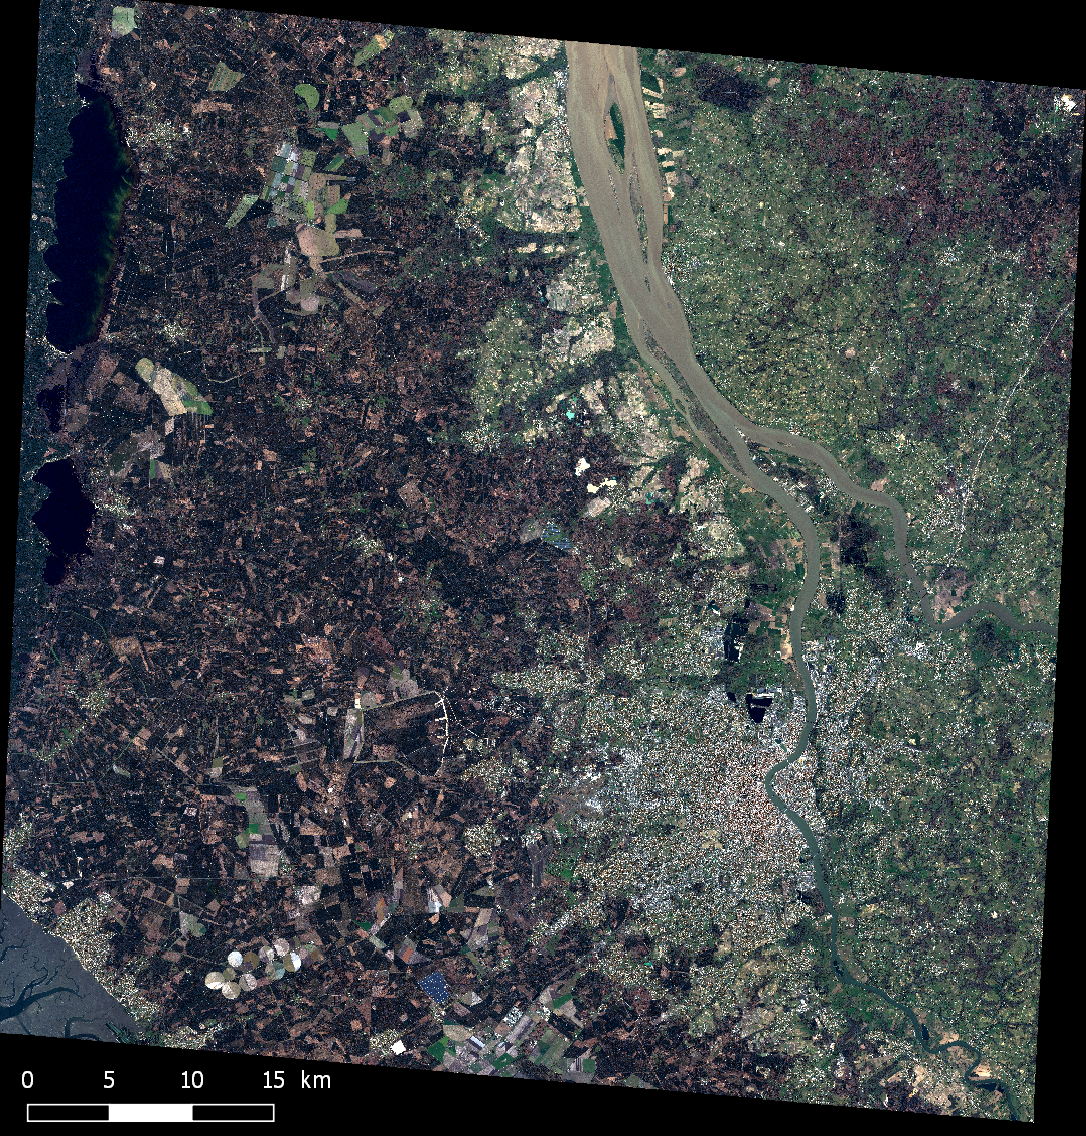
\includegraphics[width=.35\textwidth]{images/samples/gironde}
					}
					{
						\caption*{\tiny Image de la Gironde prise par SPOT en 2016: Résolution $1.5m$, $4$ canaux: \{{\color{purple!20}Infrarouge}, {\color{red}Rouge}, {\color{green}Vert}, {\color{blue}Bleu}\}.}
					}
					\ffigbox[\FBwidth]
					{
						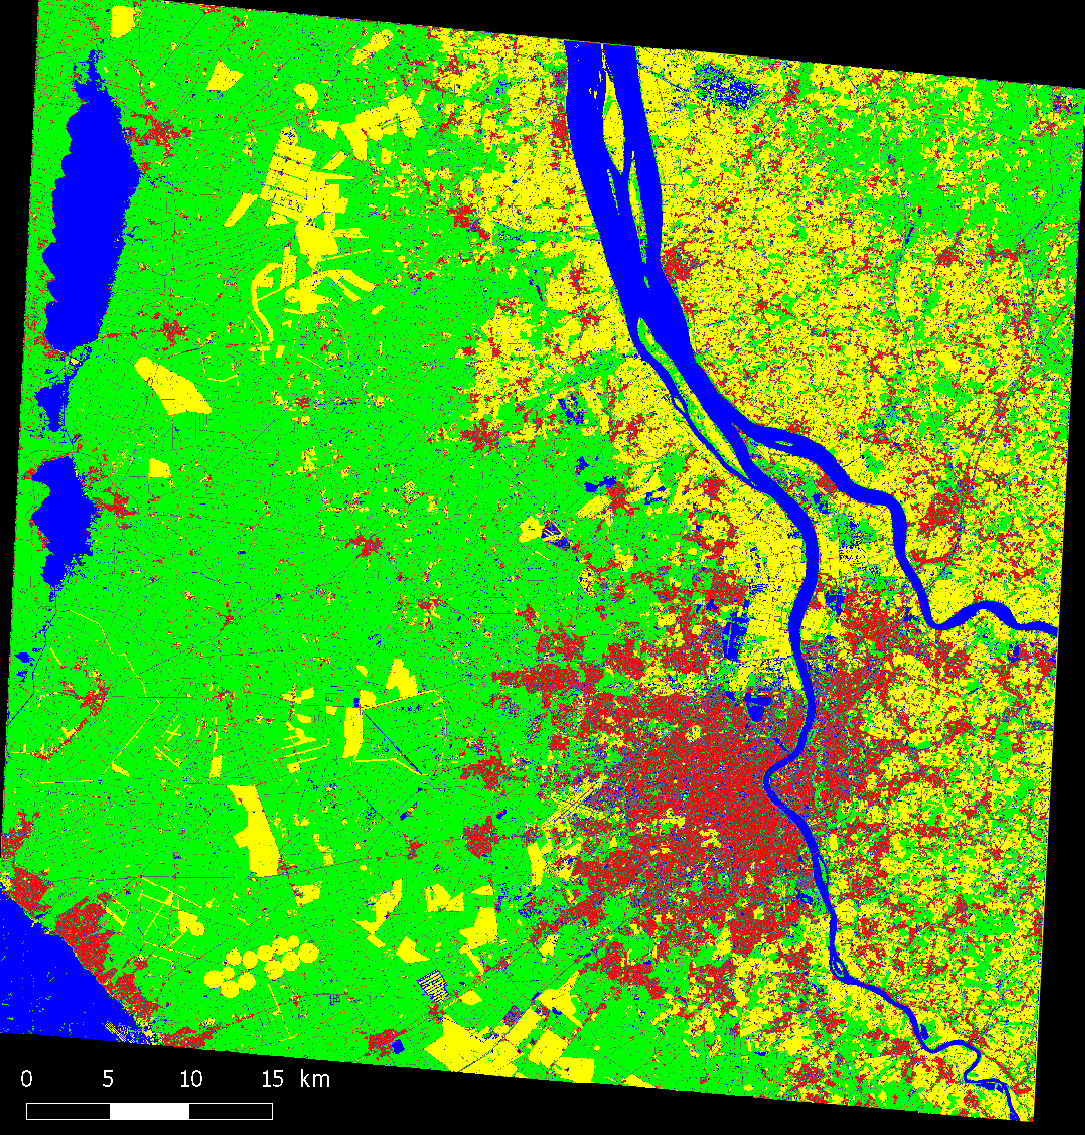
\includegraphics[width=.35\textwidth]{images/samples/gironde_classif}
					}
					{
						\caption*{\tiny Occupation des sols extraite de l'image: {\color{red}$\blacksquare$} Bâti, {\color{green}$\blacksquare$} Forêt, {\color{yellow}$\blacksquare$} Culture, {\color{gray}$\blacksquare$} Routes, {\color{blue}$\blacksquare$} Eau.}
					}
				\end{subfloatrow}
			}
			{
				\caption*{\tiny Classification appliquée pour l'Occupation des sols~\cite{postadjian2017investigating}.}
			}
		\end{figure}
	\end{frame}

	\begin{frame}{Pourquoi classifier?}
		\begin{figure}[H]
			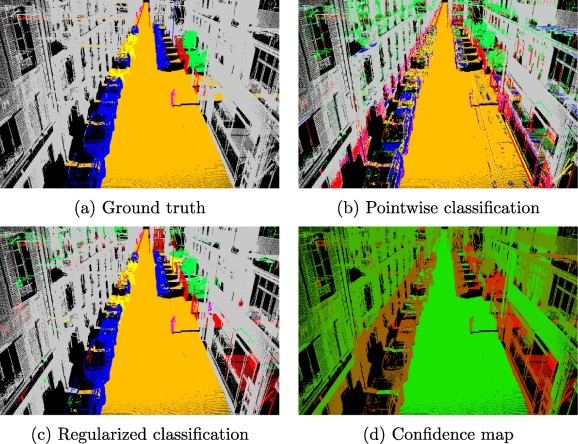
\includegraphics[width=.7\textwidth]{images/samples/pc_classification}
			\caption*{\tiny Exemple de classification de nuage de point\cite{LANDRIEU2017102}.}
		\end{figure}
	\end{frame}

	\section[SVM]{SVM}
	\begin{frame}{Curse of dimensionality}
		\begin{itemize}
			\item <1-> Si on a $n$ points à séparer, sans aucun modèle de classification, il y a un nombre exponentiel de séparations $ \frac{\vert \mathscr{P}(\{1,\dots,n\}) \vert}{2} = 2^{n-1}$ possibles $\longrightarrow$ C'est incalculable.
			\item <2-> Il faut donc un modèle de séparation qui permettra de chercher efficacement une bonne solution: Forêts Aléatoires, \textbf{SVM}, Réseaux de Neurones \dots
		\end{itemize}
	\end{frame}
	\subsection{Un peu de théorie}
		\begin{frame}{Régresser sur les probabilité: fausse bonne idée.}
			\begin{itemize}
				\item<1-> On impose un modèle de probabilité $p(y\vert x)$.
					\begin{itemize}
						\item régression de densité parametrique: Bernoulli, Poisson \dots;
						\item régression de densité non-parametrique.
					\end{itemize}
				\item<2-> \textcolor{red}{Problème: on impose trop d'hypothèses contraignantes.}
				\item<3-> Comment faire? Quels types d'hypothèse à choisir?
			\end{itemize}
		\end{frame}
		\begin{frame}{Formalisation: fonction de décision}
			\begin{itemize}
				\item<1-> On se place dans le cas de classification binaire:
					$$ X^i \in \mathbb{R}^d , \quad \forall i=1,\dots,n$$
					$$ Y^i \in \{-1, +1\} , \quad \forall i=1,\dots,n$$
					$$\eta(x) = p(y = 1 \vert x) = 1 - p(y = -1 \vert x), \quad \forall x \in \mathbb{R}^d$$
				\item<2-> On cherche une fonction de décision $D$ comme suit:
				\begin{align*}
					D: \mathbb{R}^d &\rightarrow \{-1, +1\} \\
					x &\mapsto D(x)
				\end{align*}
				\item<3-> On définit le regret, ou risque, d'une fonction de décision $D$ par:
				\begin{equation}
					R(D) \triangleq \mathbb{E}_{X,Y}(\mathbb{1}(D(X)\neq Y))
				\end{equation}
				\item<4-> Cette fonction calcule la mesure de l'espace d'attributs où $D(x) \neq y$:
				\begin{align*}
					R(D) &= \mathbb{P}(\{D(X)\neq Y\})\\
						 &= \sum_{y\in \{-1, 1\}} \int_{x \in \mathbb{R}^d} \mathbb{1}(D(x)\neq y) p(dx, y)
				\end{align*}
			\end{itemize}
		\end{frame}
		\begin{frame}{Fonction de décision optimal}
			\begin{itemize}
				\item<1-> Le "décideur" optimal $D^*$ donne le regret $R(D^*)$ minimal:
					  \begin{equation}
						  D^* \triangleq \arg \min_{D} R(D) 
					  \end{equation}
				\item<2-> On appelle cette fonction la fonction de décision de Bayes. On prouve que:
					  \begin{equation}
						D^*(x) \triangleq 2.\mathbb{1}(\eta(x) > \frac{1}{2}) - 1
					  \end{equation}
				\item<3-> En pratique, on ne connait pas $\eta: \mathbb{R}^d \rightarrow [0,1]$.
			\end{itemize}
		\end{frame}

		\begin{frame}{Apprentissage de séparateur}
			\begin{itemize}
				\item<1-> On évite de modéliser $\eta$ sur tout l'espace d'attributs $\mathbb{R}^d$.
				\item<2-> Il est plus judicieux de modèliser $\eta$ sur les points $x$ où:
						\begin{equation*}
							\eta(x) = \frac{1}{2}
						\end{equation*}
				\item<3->  Cela revient à étudier ce qu'on appelle un séparateur; i.e. la courbe qui vérifie:
					\begin{equation}
						\mathscr{S}_{binary} \triangleq \{X \in \mathbb{R}^d: \eta(x) = \frac{1}{2} \}
					\end{equation}
			\end{itemize}
		\end{frame}

		\begin{frame}{Séparateur: illustration}
			\begin{figure}[H]
				\includestandalone[mode=buildnew, width=.5\textwidth]{scatter_separators}
				\caption*{\tiny Séparateurs possibles des données. $\mathscr{S}_1$ est un exemple de séparateur courbe alors que $\mathscr{S}_2$ est un séparateur linéaire.}
			\end{figure}
		\end{frame}

		\begin{frame}{Choix du séparateur}
			\begin{itemize}
				\item  Il y a une infinité de modèle de $D$ possible.
				\item  Un choix naïf serait de donner, pour chaque instance d'entraînement $X^i$, la valeur qui lui est associé $Y^i$, et pour toute autre valeur $x$ une classe de façon aléatoire:
				\begin{equation*}
					D_n(x) = \sum_{i=1,\dots,n} Y^i . \delta_{X^i}(x) + b . \mathbb{1}_{x \notin \{X^i, \forall i=1,\dots,n\}}
				\end{equation*}
				où: $b \sim \mathscr{B}(0.5)$ est une valeur aléatoire qui suit une loi de Bernoulli avec paramètre $0.5$.
				\item Cependant, ce classifieur n'a aucun pourvoir de généralisation. En effet:
				\begin{gather*}
					\widetilde{x} := \sum_{i=1,\dots,n} X^i \notin \{X^i, \forall i=1,\dots,n\} \\
					\Rightarrow D_n(\widetilde{x}) \sim \mathscr{B}(0.5)
				\end{gather*}
				\item  On réduit, dans le cadre du cours, le choix des séparateurs à ceux qui sont linéaires:
				\begin{align*}
					D_{\textbf{w}, b}: \mathbb{R}^d &\rightarrow \{-1, +1\} \\
					\textbf{x} &\mapsto D_{\textbf{w}, b}(\textbf{x}) = 2.\mathbb{1}(\textbf{w}.\textbf{x} + b > 0) - 1
				\end{align*}
			\end{itemize}
		\end{frame}

	\subsection[linear]{SVM linéaire}
		\begin{frame}{Mais c'est quoi donc ce SVM?}
			\begin{itemize}
				\item  SVM\@: Support Vector Machines.
				\item  C'est quoi donc un vecteur support?
				\item  Quelle est la relation avec les séparateurs linéaires?
			\end{itemize}
		\end{frame}

		\begin{frame}{SVM\@: maximiser la marge.}
			\begin{figure}[H]
				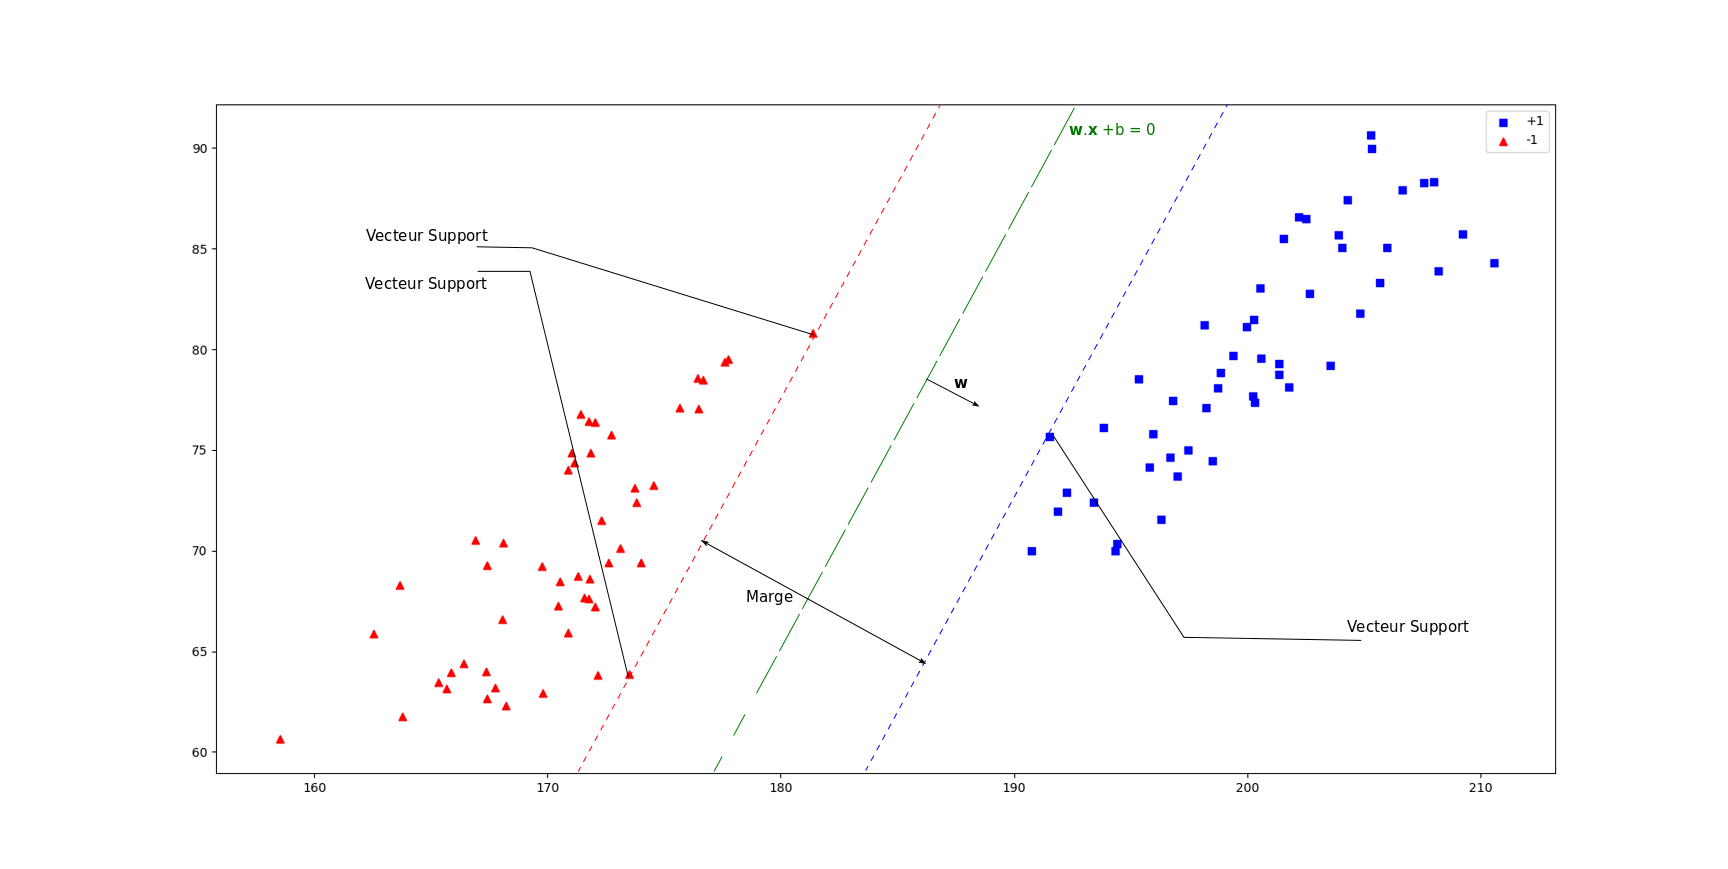
\includegraphics[width=\textwidth]{images/samples/svm}
				\caption*{ Le séparateur linéaire SVM.}
			\end{figure}
		\end{frame}

		\begin{frame}{SVM\@: maximiser la marge.}
			\begin{itemize}
				\item  Le but du SVM est de maximiser la marge~\cite{vapnik1998statistical}.
				\item  On remarque que:
				\begin{gather*}
					(\textbf{w}, b) \in \{\omega \in \mathbb{R}^d : \omega.\textbf{x} + b = 0\} \\
					\Rightarrow
					(\lambda . \textbf{w}, \lambda.b) \in \{\omega \in \mathbb{R}^d : \omega.\textbf{x} + b = 0\}\quad, \forall \lambda \in \mathbb{R}\setminus\{0\}
				\end{gather*}
				\item  Il y a donc une infinité de solutions possibles. On prend donc la solution $\textbf{w}$ qui permet d'avoir:
				\begin{align}
					\textbf{w}.\textbf{x}_{\color{blue}+} + b &= {\color{blue}+}1 \\
					\textbf{w}.\textbf{x}_{\color{red}-} + b &= {\color{red}-}1
				\end{align}
				où:
				\begin{itemize}
					\item[{\color{blue}+}] $\textbf{x}_{\color{blue}+}$ correspond aux vecteurs supports positifs (i.e. $Y={\color{blue}+}1$).
					\item[{\color{red}---}] $\textbf{x}_{\color{red}-}$ correspond aux vecteurs supports négatifs (i.e. $Y={\color{red}-}1$).
				\end{itemize}
			\end{itemize}
		\end{frame}

		\begin{frame}[plain]{SVM\@: maximiser la marge}
			\begin{figure}[H]
				\includestandalone[mode=buildnew, width=.75\textwidth]{svm_separable}
				\caption*{\tiny Le séparateur linéaire SVM.}
			\end{figure}
		\end{frame}

		\begin{frame}{La marge}
			\begin{itemize}
				\only<1>{
					\item  La marge est la longueur de la projection orthogonal de $(\textbf{x}_+ - \textbf{x}_-)$ sur la droite porter par $\textbf{w}$:
						\begin{align*}
						M &= \frac{\textbf{w}}{\vert\vert \textbf{w} \vert\vert}.(\textbf{x}_+ - \textbf{x}_-) \\
						&= \frac{\textbf{w}.\textbf{x}_+ - \textbf{w}.\textbf{x}_-}{\vert\vert \textbf{w} \vert\vert}\\
						&= \frac{\textbf{w}.\textbf{x}_+ + b - (\textbf{w}.\textbf{x}_- + b)}{\vert\vert \textbf{w} \vert\vert}\\
						&= \frac{2}{\vert\vert \textbf{w} \vert\vert}
						\end{align*}
				}
				\item<2-> La marge est la longueur de la projection orthogonal de $(\textbf{x}_+ - \textbf{x}_-)$ sur la droite porter par $\textbf{w}$:
					\begin{equation}
						M = \frac{2}{\vert\vert \textbf{w} \vert\vert}
					\end{equation}
				\item<2->  Le problème posé par le SVM est donc formulé comme suit:
				\begin{equation}
					\begin{aligned}
					& \max_{\textbf{w}}
					& & \frac{2}{\vert\vert \textbf{w} \vert\vert} \\
					& \text{sous contrainte}
					& & \begin{cases}
						\textbf{w}.\textbf{X}^i + b \leq -1 & Y^i = -1 \\
						\textbf{w}.\textbf{X}^i + b \geq 1 & Y^i = 1
					\end{cases} \; \forall i = 1, \dots, n.
					\end{aligned}
				\end{equation}
				\item<2->  Ou encore:
				\begin{equation}
					\begin{aligned}
					& \min_{\textbf{w}}
					& & {\vert\vert \textbf{w} \vert\vert}^2 \\
					& \text{sous contrainte}
					& & Y^i.(\textbf{w}.\textbf{X}^i + b) \geq 1 \; \forall i = 1, \dots, n.
					\end{aligned}
				\end{equation}
			\end{itemize}
		\end{frame}

		\begin{frame}{Cas non séparable.}
			\begin{figure}[H]
				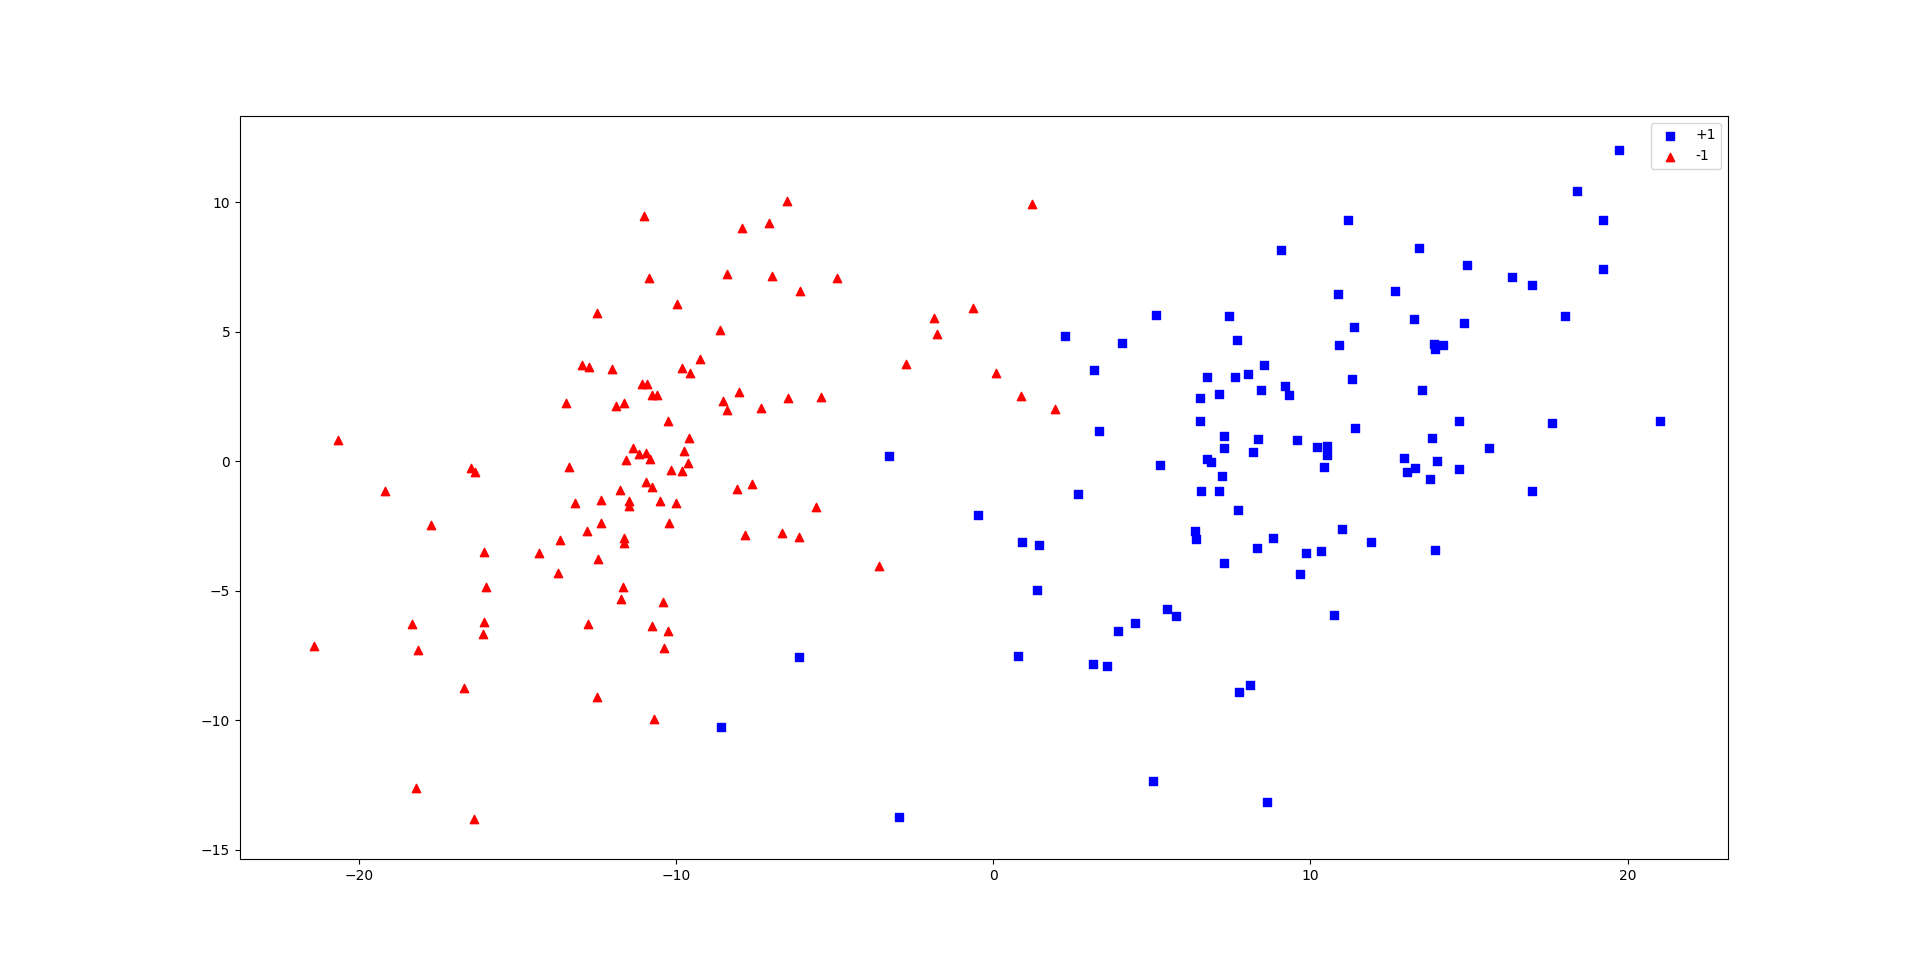
\includegraphics[width=\textwidth]{images/samples/non_separable}
				\caption*{\label{fig::non_sep} Le séparateur linéaire SVM.}
			\end{figure}
		\end{frame}

		\begin{frame}{Cas non séparable.}
			\begin{figure}[H]
				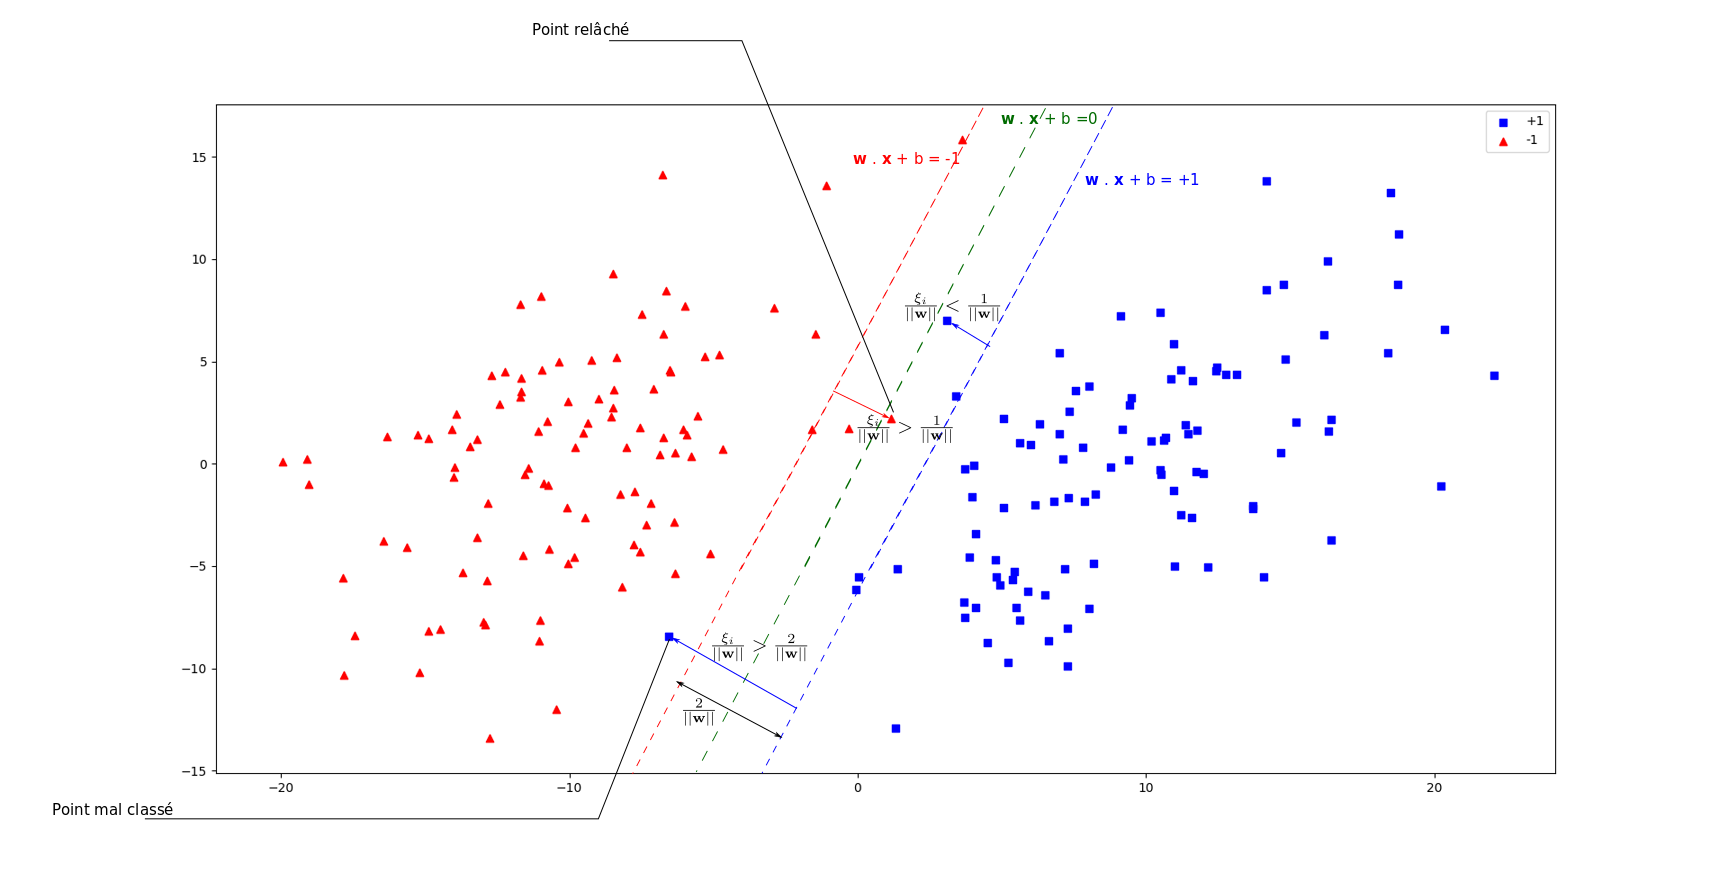
\includegraphics[width=\textwidth]{images/samples/stable_margin}
				\caption*{\label{fig::stable_margin} La marge du séparateur linéaire SVM.}
			\end{figure}
		\end{frame}

		\begin{frame}{Cas non séparable.}
			\begin{itemize}
				\only<1-8>{
					\item<1->  On lâche du ``mou'': On accepte des fois que
						$$\exists k \; Y^k.(\textbf{w}.\textbf{X}^k + b) < 1$$
					\item<2->  On écrire autrement:
						\begin{equation}
							\forall i=1,\dots,n \quad \exists \xi_i \geq 0 \quad Y^i.(\textbf{w}.\textbf{X}^i + b) \geq 1 - \xi_i
						\end{equation}

					\item<3->  Il y a donc quatres cas pour $ \xi_i $:
					\begin{itemize}
						\item<4-> $\xi_i = 0 \Rightarrow$ Point bien classé;
						\item<5-> $0 < \xi_i \leq 1 \Rightarrow$ Point situé dans la marge: bien classé mais moins sûr;
						\item<6-> $1 < \xi_i < 2 \Rightarrow$ Point de l'autre côté de la ligne séparatrice mais dans la marge: donc mal classé et pas très sûr;
						\item<7-> $2 \leq \xi_i \Rightarrow$ Point non séparable, il dépasse l'autre limite de marge: sûrement mal classé;
					\end{itemize}

					\item<8->  Dans le cas ou le problème n'est pas séparable linéairement, on peut déduire que
					$\exists i_0 \in \{1, \dots, n\}, \quad 1 < \xi_{i_0}$
				}

				\item<9->  N'importe quel droite peut ainsi séparer les données. Les différents $\xi_i$ peuvent donc être très grand. Par conséquent, il faut les pénaliser au moment de l'optimisation. Le problème devient:
					\begin{equation}
						\begin{aligned}
						& \min_{\textbf{w}, \xi_1,\dots,\xi_n \in \mathbb{R}^+}
						& & {\vert\vert \textbf{w} \vert\vert}^2 + C.\sum_{i=1,\dots,n}\xi_i\\
						& \text{sous contrainte}
						& & Y^i.(\textbf{w}.\textbf{X}^i + b) \geq 1 - \xi_i , \forall i = 1, \dots, n.
						\end{aligned}
					\end{equation}
			\end{itemize}
		\end{frame}

		\begin{frame}{Cas de la constante de régularisation}
			\begin{itemize}
				\item<1->  $C \ll 1 \Longrightarrow$ moins de pénalisation sur les variables de ressort $\Longrightarrow$ marge très grande, plus de généralisation;
				\item<2->  $C \gg 1 \Longrightarrow$ plus de pénalisation sur les variables de ressort $\Longrightarrow$ marge serrée, moins de généralisation;
				\item<3->  $C=\infty \Longrightarrow$ pénalisation complète sur les variables de ressort $\Longrightarrow$ marge dure: c'est la première version de SVM qu'on a vu.
			\end{itemize}
		\end{frame}
		\begin{frame}{Optimization Quadratique! Peut-on faire mieux?}
			\begin{itemize}
				\item<1->  Problème primal (Quadratique):
				\begin{equation}
					\begin{aligned}
					& \min_{\textbf{w}, \xi_1,\dots,\xi_n \in \mathbb{R}^+}
					& & {\vert\vert \textbf{w} \vert\vert}^2 + C.\sum_{i=1,\dots,n}\xi_i \\
					& \text{sous contrainte}
					& & Y^i.(\textbf{w}.\textbf{X}^i + b) \geq 1 - \xi_i , \forall i = 1, \dots, n.
					\end{aligned}
				\end{equation}
				\item<2->  Problème dual:
				\begin{equation}
					\begin{aligned}
					& \max_{0 \leq \alpha_i \leq C ,\forall i=1,\dots,n}
					& & \sum_{i=1,\dots,n} \alpha_i - \frac{1}{2}.\sum_{l,p=1,\dots,n}\alpha_l.\alpha_p.Y^l.Y^p.<X^l,X^p>\\
					& \text{sous contrainte}
					& & \sum_{i=1,\dots,n}Y^i.\alpha_i=0
					\end{aligned}
				\end{equation}
				où: $<x, x'>$ est le produit scalaire des deux vecteurs $\textbf{x}$ et $\textbf{x'}$ noté aussi précédemment $\textbf{x}.\textbf{x'}$.
			\end{itemize}
		\end{frame}
		\begin{frame}{Algorithmes en Pratiques}

			On admet que la résolution d'un problème est équivalente à la résolution de l'autre.
			\begin{itemize}
				\item  Problème Primal: Descente de Gradient Stochastique~\cite{bottou2010} (SGD).
				\item  Problème Dual: Sequential minimal Optimization (SMO)~\cite{platt1998sequential} et dérivés.
			\end{itemize}
		\end{frame}
	\subsection[kernel]{Kernel SVM}

	\begin{frame}{Changement d'espace}
		\begin{figure}[H]
			\begin{center}
				\includestandalone[mode=buildnew, width=.6\textwidth]{scatter_circles}
				\caption*{\label{fig::circles_3} Quelle transformation à appliquer pour obtenir des instances séparables linéairement?}
			\end{center}
		\end{figure}
	\end{frame}
	\begin{frame}[plain]{Changement d'espace}
		\begin{itemize}
			\item  Trouver la transformation $\Phi$:
			\begin{figure}[H]
				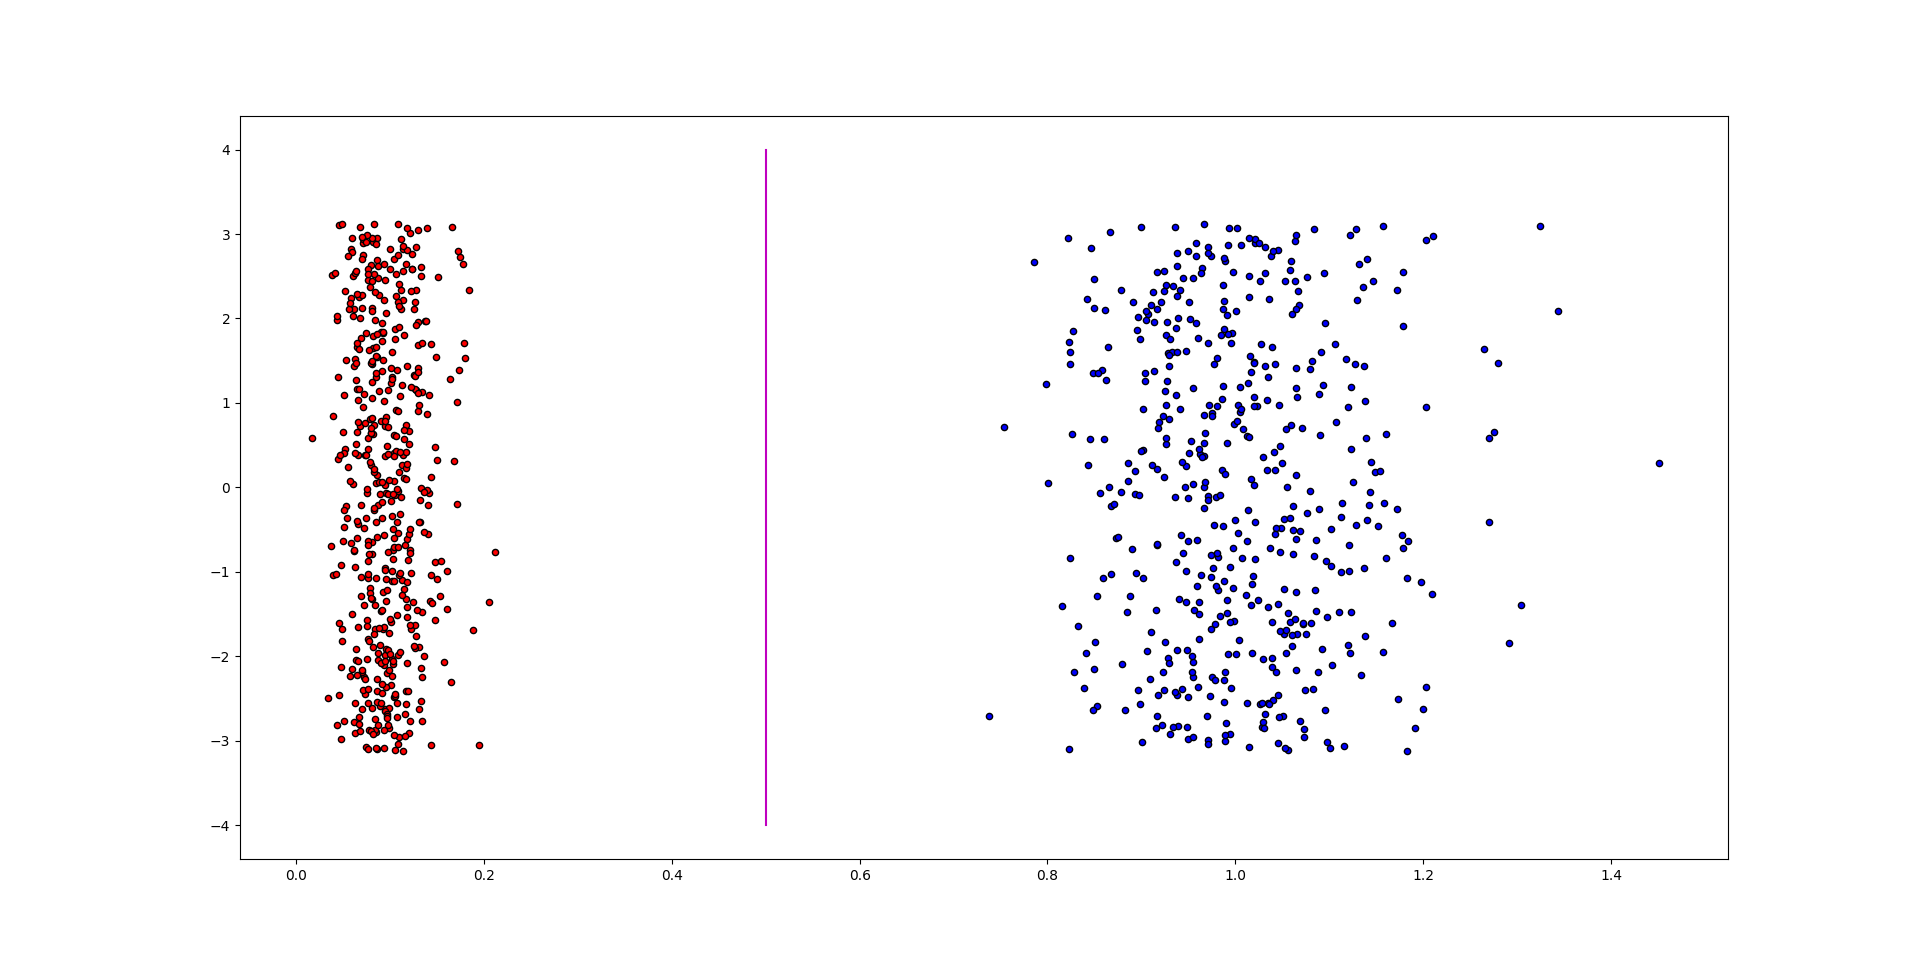
\includegraphics[width=.7\textwidth]{images/samples/separation_pol}
				\caption*{\label{fig::kernel_polar} Exemple de changement d'espace avec une transfomation $\Phi$.}
			\end{figure}
			\item En coordonnées polaires:
			\begin{align*}
				\Phi: \mathbb{R}^2 &\rightarrow \mathbb{R}^2 \\
				\begin{pmatrix}
					x \\
					y
				\end{pmatrix} &\mapsto \begin{pmatrix}
					x^2 + y^2 \\
					\arctan(x/y)
				\end{pmatrix}
			\end{align*}
		\end{itemize}
	\end{frame}
	\begin{frame}{Changement d'espace}
		\begin{itemize}
			\item  Trouver la transformation $\Phi$:
			\begin{figure}[H]
				\ffigbox[\FBwidth]
				{
					\begin{subfloatrow}[2]
						\ffigbox[\FBwidth]
						{
							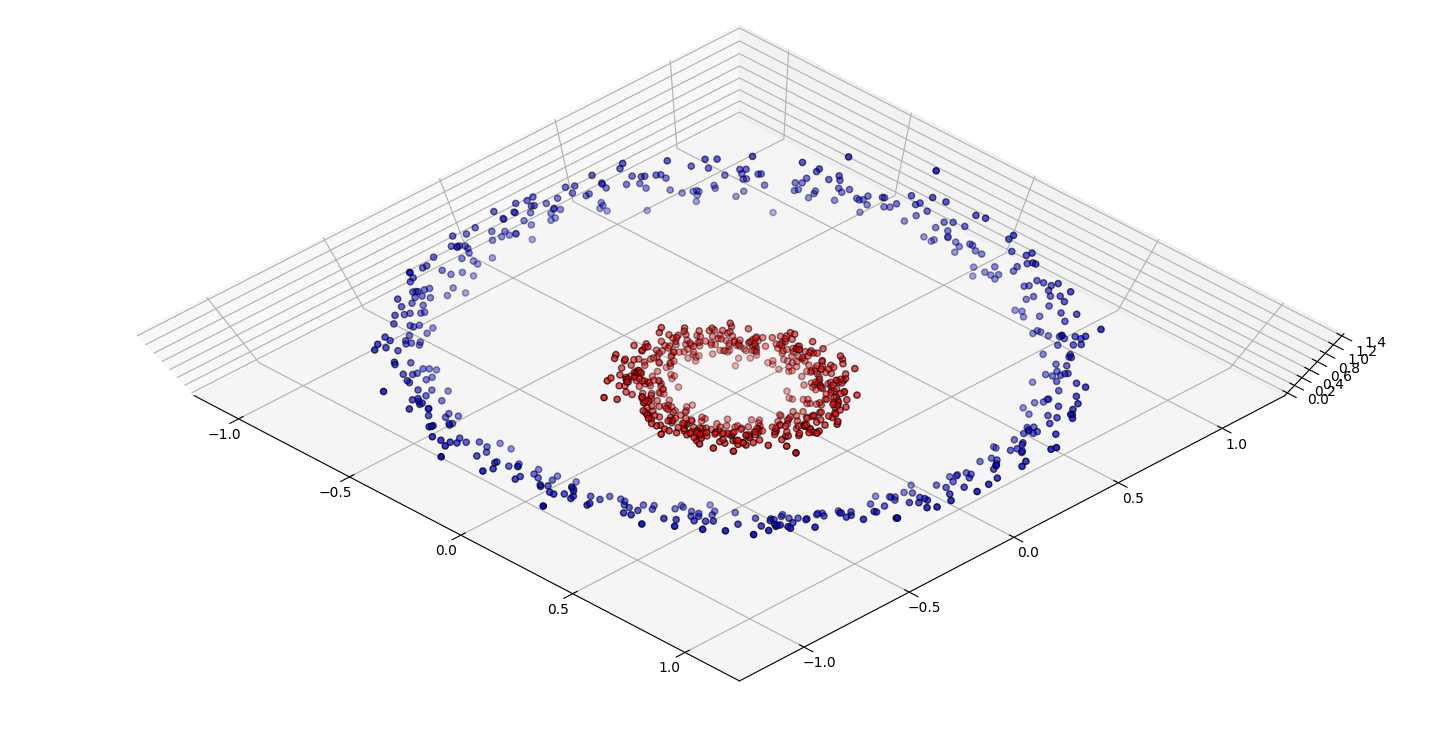
\includegraphics[width=.45\textwidth]{images/samples/map_L_2_separation}
						}
						{
							\caption*{Vue de haut.}
						}
						\ffigbox[\FBwidth]
						{
							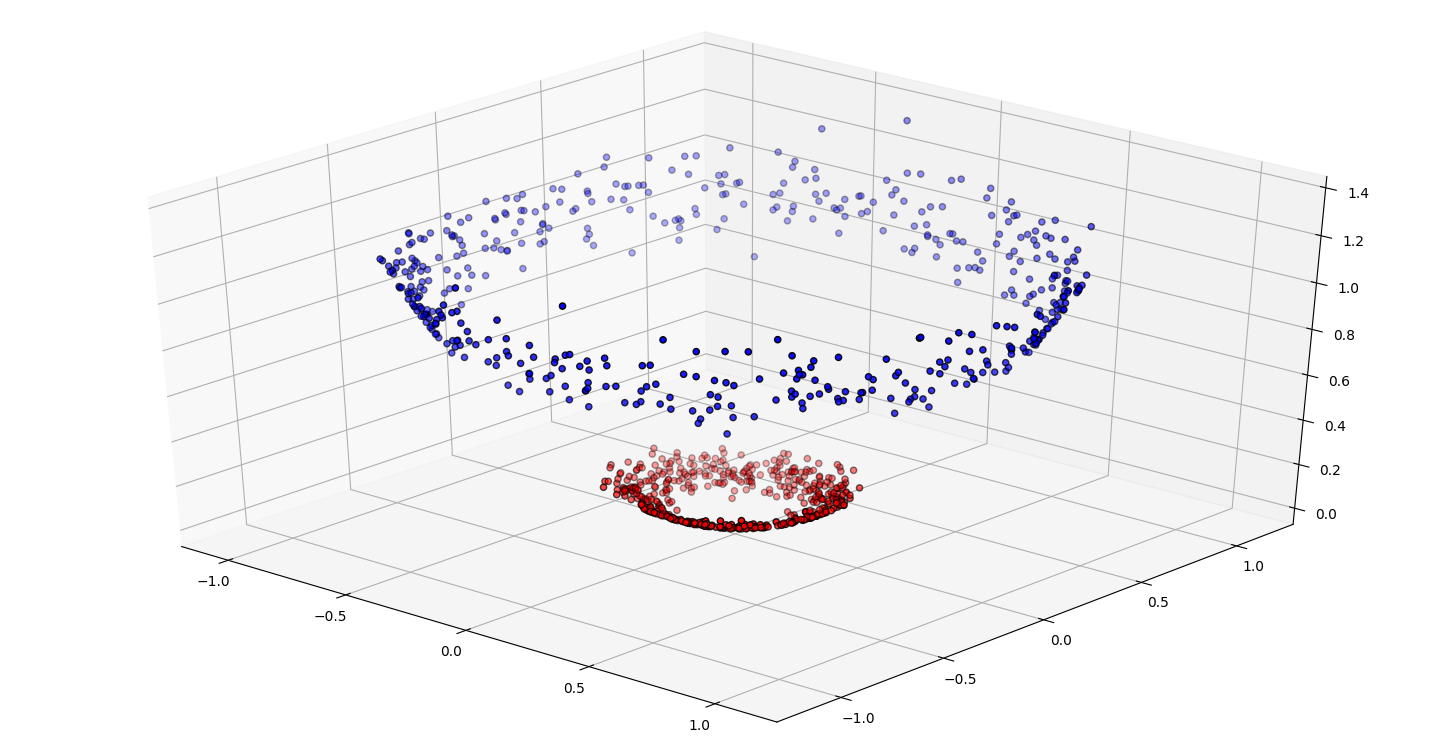
\includegraphics[width=.45\textwidth]{images/samples/map_L_2_separation_1}
						}
						{
							\caption*{Vue transversale.}
						}
					\end{subfloatrow}
				}
				{
					\caption*{  Exemple de changement d'espace avec une transfomation $\Phi$.}
				}
			\end{figure}
		\end{itemize}
	\end{frame}
	\begin{frame}{Changement d'espace}
		\begin{itemize}
			\item <1-> Séparation linéaire dans le nouveau espace:
			\begin{figure}[H]
				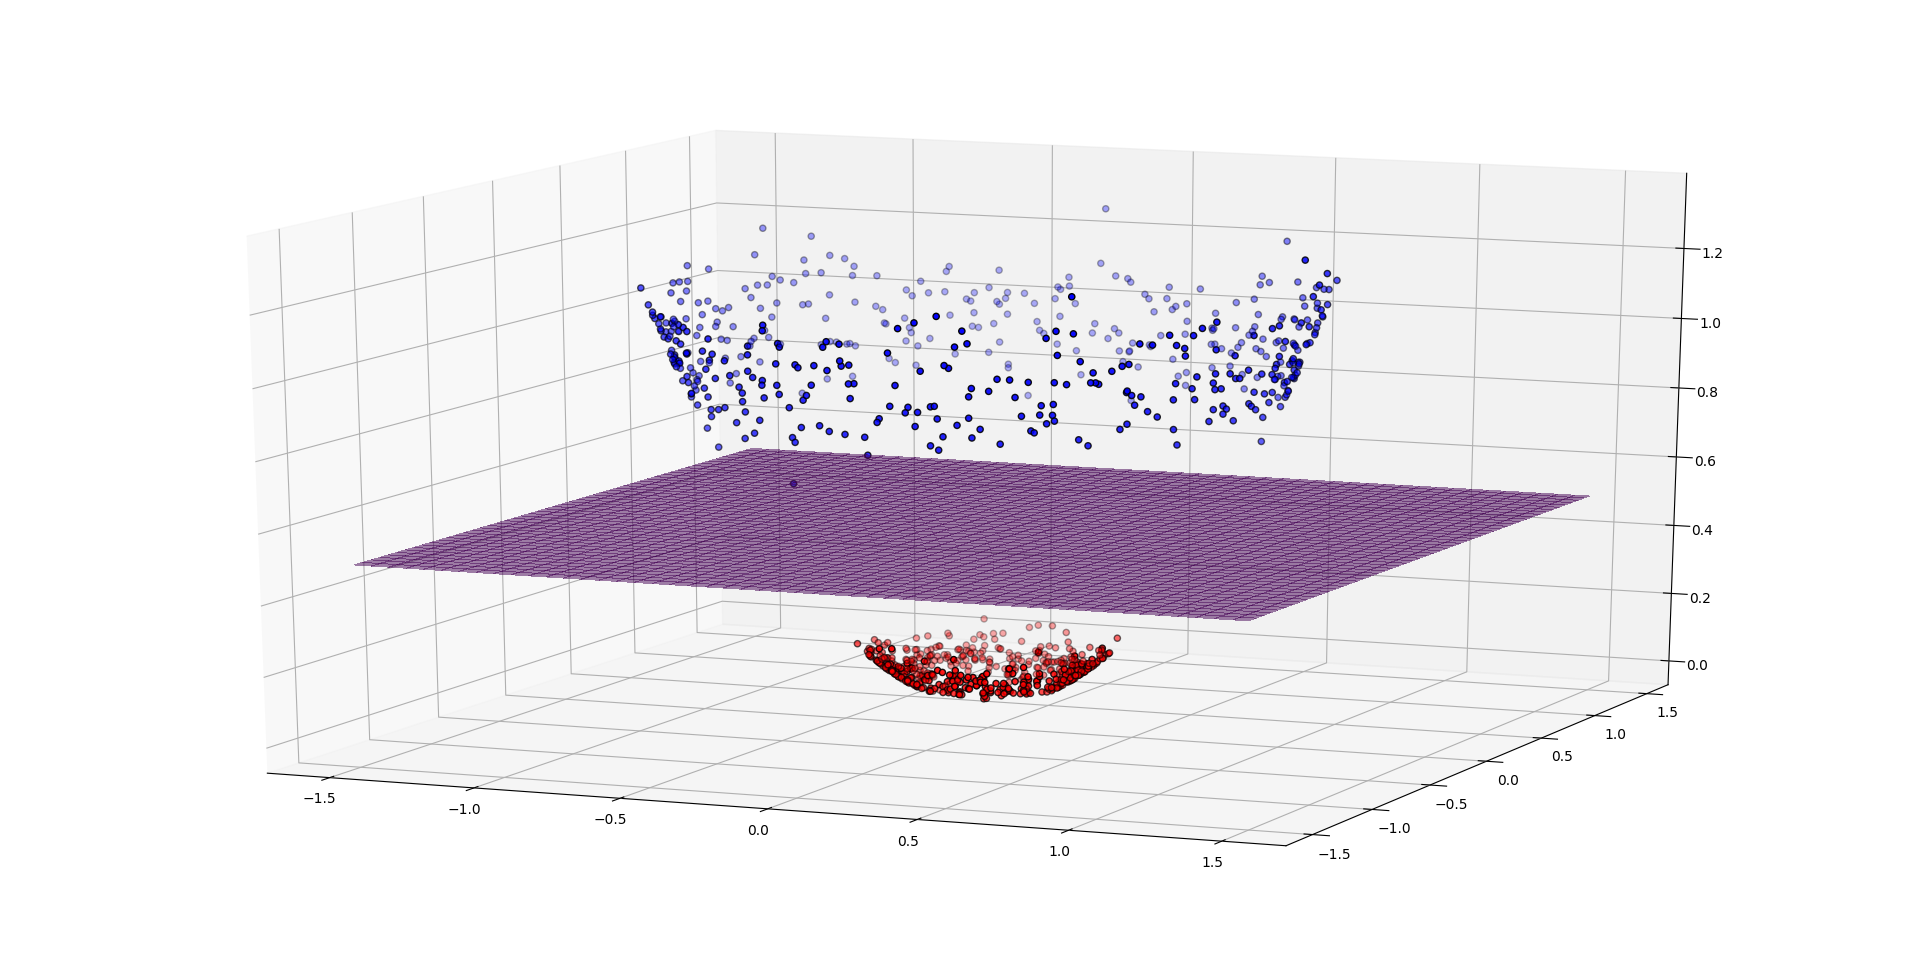
\includegraphics[width=.5\textwidth]{images/samples/separation_x_2_y_2}
				\caption*{ Hyperplan séparant les deux classes dans le nouveau espace.}

			\end{figure}
			\item <2-> \begin{align*}
				\Phi: \mathbb{R}^2 &\rightarrow \mathbb{R}^3 \\
				\begin{pmatrix}
					x \\
					y
				\end{pmatrix} &\mapsto \begin{pmatrix}
					x \\
					y \\
					x^2 + y^2
				\end{pmatrix}
			\end{align*}
		\end{itemize}
	\end{frame}
	\begin{frame}{Changement d'espace}
		\begin{itemize}
			\item  Trouver la transformation $\Phi$:
			\begin{figure}[H]
				\ffigbox[\FBwidth]
				{
					\begin{subfloatrow}[2]
						\ffigbox[\FBwidth]
						{
							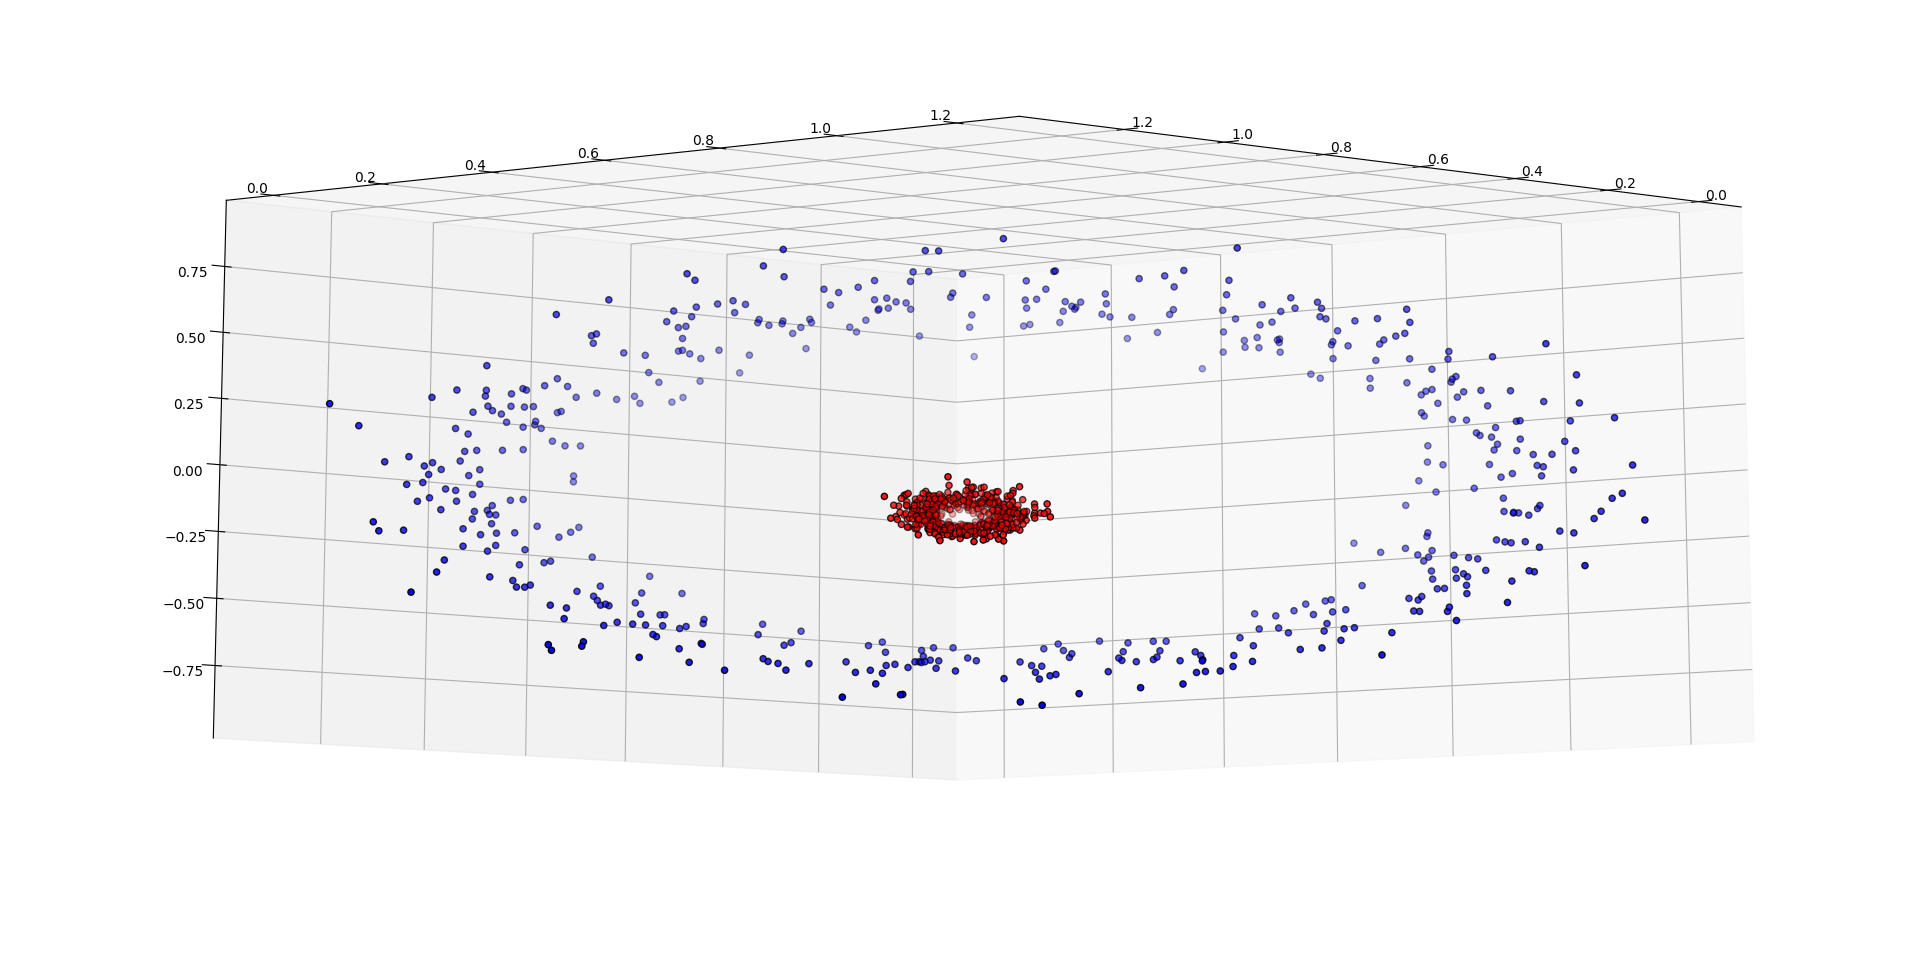
\includegraphics[width=.45\textwidth]{images/samples/separation_pol_2_1}
						}
						{
							\caption*{Vue de haut.}
						}
						\ffigbox[\FBwidth]
						{
							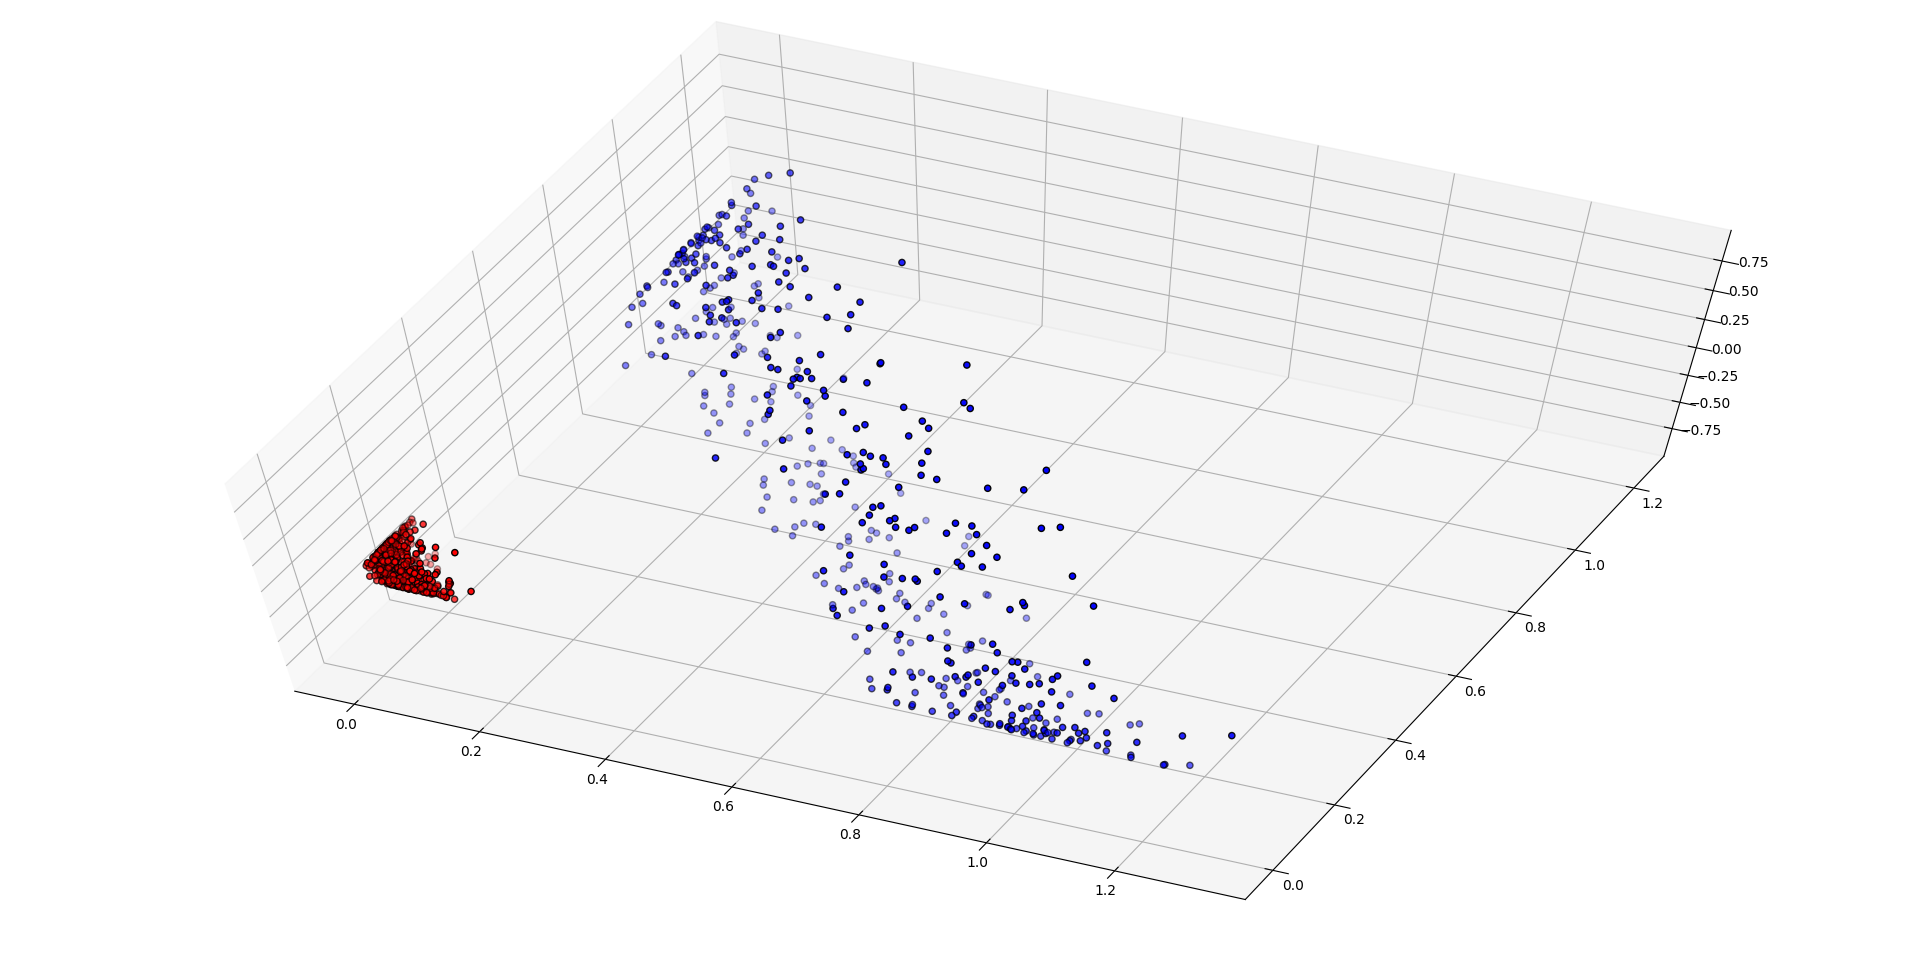
\includegraphics[width=.45\textwidth]{images/samples/separation_pol_2_2}
						}
						{
							\caption*{Vue transversale.}
						}
					\end{subfloatrow}
				}
				{
					\caption*{Exemple de changement d'espace avec une transfomation $\Phi$.}
				}
			\end{figure}
		\end{itemize}
	\end{frame}
	\begin{frame}[plain]{Changement d'espace}
		\begin{itemize}
			\item <1-> Séparation linéaire dans le nouveau espace:
			\begin{figure}[H]
				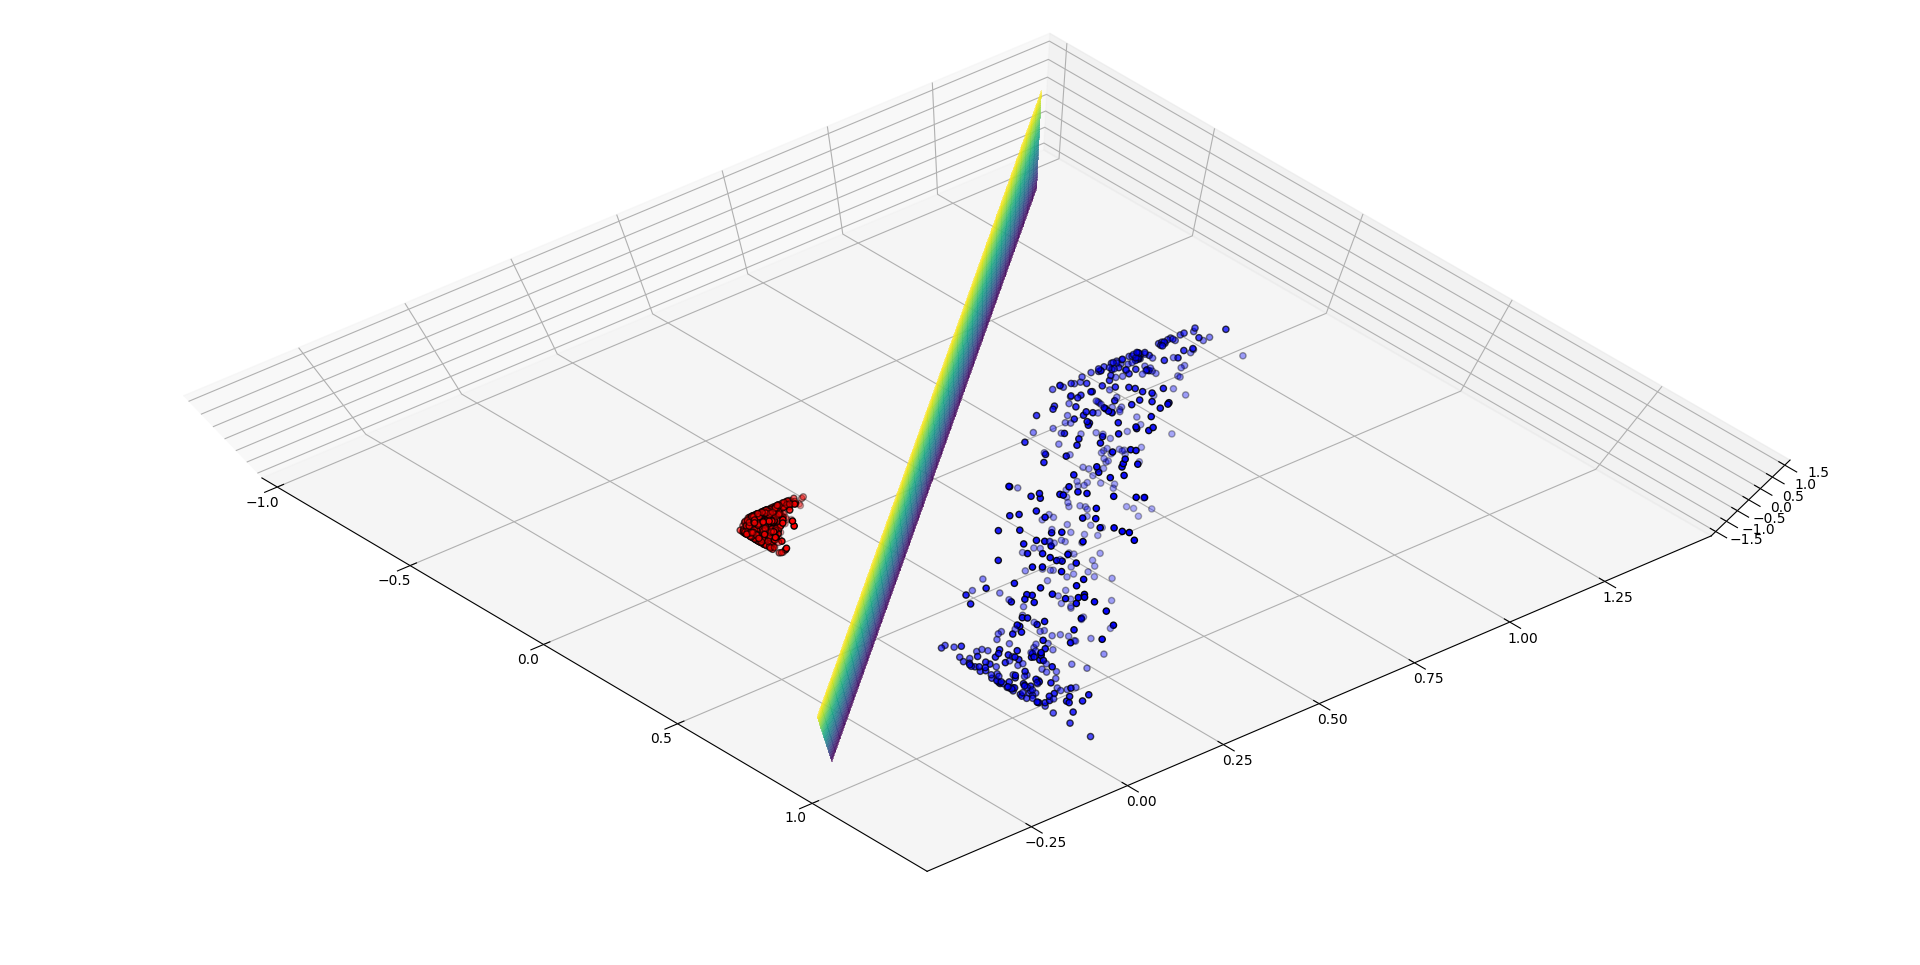
\includegraphics[width=.7\textwidth]{images/samples/separation_pol_2_3}
				\caption*{\label{fig::pol_take_3} Hyperplan séparant les deux classes dans le nouveau espace.}

			\end{figure}
			\item <2-> Transformation \textit{polynomiale}:
			\begin{align*}
				\Phi: \mathbb{R}^2 &\rightarrow \mathbb{R}^3 \\
				\begin{pmatrix}
					x \\
					y
				\end{pmatrix} &\mapsto \begin{pmatrix}
					x^2 \\
					y^2 \\
					\sqrt{2}.x.y
				\end{pmatrix}
			\end{align*}
		\end{itemize}
	\end{frame}
	\begin{frame}{Changement d'espace}
		\begin{itemize}
			\item  Le but du changement d'espace est de pouvoir séparer linéairement le problème dans un nouvel espace où les distances Euclidiennes ont un sens;
			\item  On transforme donc les observations avec une application comme suit:
			\begin{align*}
				\Phi: \mathbb{R}^d &\rightarrow \mathbb{R}^p \\
				X &\mapsto \Phi(X)
			\end{align*}
			où $p\geq d$.
		\end{itemize}
	\end{frame}

	\begin{frame}{Que devient donc le problème d'optimisation:}
		\begin{itemize}
			\item  Problème primal:
			\begin{equation}
				\begin{aligned}
				& \min_{\textbf{w}, \xi_1,\dots,\xi_n \in \mathbb{R}^+}
				& & {\vert\vert \textbf{w} \vert\vert}^2 + C.\sum_{i=1,\dots,n}\xi_i \\
				& \text{sous contrainte}
				& & Y^i.(\textbf{w}.\Phi(\textbf{X}^i) + b) \geq 1 - \xi_i , \forall i = 1, \dots, n.
				\end{aligned}
			\end{equation}
			\item  Problème dual:
			\begin{equation}
				\begin{aligned}
				& \max_{0 \leq \alpha_i \leq C ,\forall i=1,\dots,n}
				& & \sum_{i=1,\dots,n} \alpha_i - \frac{1}{2}.\sum_{l,p=1,\dots,n}\alpha_l.\alpha_p.Y^l.Y^p.<\Phi(X^l),\Phi(X^p)>\\
				& \text{sous contrainte}
				& & \sum_{i=1,\dots,n}Y^i.\alpha_i=0
				\end{aligned}
			\end{equation}
			\item  Que peut on relever sur ce dernier problème d'optimisation?
		\end{itemize}
	\end{frame}

	\begin{frame}{Kernel Trick}
		\begin{itemize}
			\item <1-> La transformation $\Phi$ ne nous intéresse pas, en soi;
			\item <2-> Ce sont les distances Euclidienne dans le nouveau espace:
			$$\forall X, Y \in \mathbb{R}^d$$
			\begin{align*}
				\vert\vert\Phi(X) - \Phi(Y)\vert\vert_2^2 &= \vert\vert\Phi(X)\vert\vert_2^2 + \vert\vert\Phi(Y)\vert\vert_2^2 - 2 \vert\vert\Phi(X)\vert\vert.\vert\vert\Phi(Y)\vert\vert_2^2 \\
				 &= <\Phi(X),\Phi(X)> + <\Phi(Y),\Phi(Y)> - 2 <\Phi(X),\Phi(Y)>
			\end{align*}
			\item <3-> Il suffit de calculer le nouveau produit scalaire:
			\begin{equation}
				\forall X, Y \in \mathbb{R}^d \quad k(X, Y) \triangleq <\Phi(X),\Phi(Y)>
			\end{equation}
			où:
			\begin{align*}
				k: \mathbb{R}^d \times \mathbb{R}^d &\rightarrow \mathbb{R}^+ \\
				(X, Y) &\mapsto k(X, Y)
			\end{align*}
			est ce qu'on appelle le \textit{kernel}.
		\end{itemize}
	\end{frame}

	\begin{frame}{Kernels Usuels}
		\begin{itemize}
			\item  Radial Basis Function (RBF):
			\begin{equation}
				k_{\gamma}(x,y) = \exp{-\gamma.\vert\vert x-y \vert\vert^2}
			\end{equation}
			\item  Kernel Polynomial:
			\begin{equation}
				k_{\gamma, c}(x,y) = (x^t.y + c)^{\gamma}
			\end{equation}
			\item  Kernel Sigmoïde:
			\begin{equation}
				k_{\gamma, c}(x,y) = \gamma.\tanh(x^t.y + c)
			\end{equation}
		\end{itemize}
	\end{frame}

	\begin{frame}[plain]{Kernels Usuels}
		\begin{figure}[H]
			\ffigbox[\FBwidth]
			{
				\begin{subfloatrow}[2]
					\ffigbox[\FBwidth]
					{
						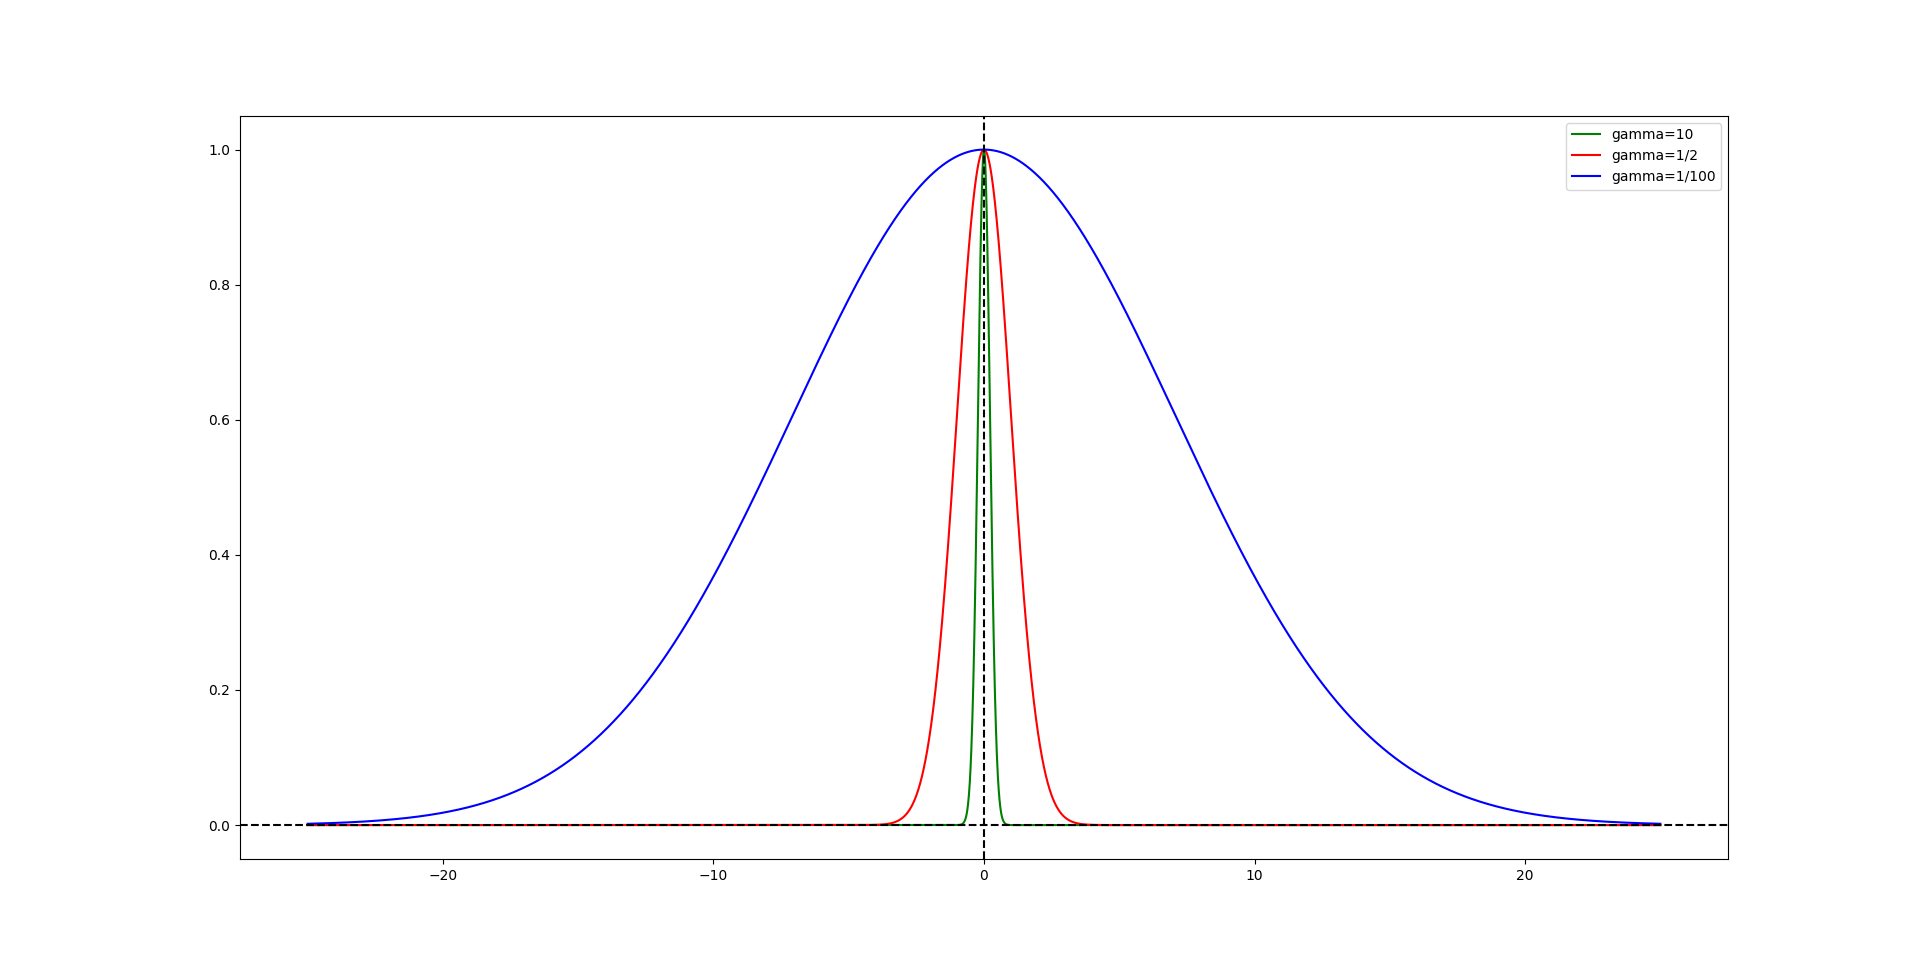
\includegraphics[width=.45\textwidth]{images/samples/rbfs}
					}
					{
						\caption*{RBF avec différentes valeurs de $\gamma$.}\label{fig::rbfs}
					}
					\ffigbox[\FBwidth]
					{
						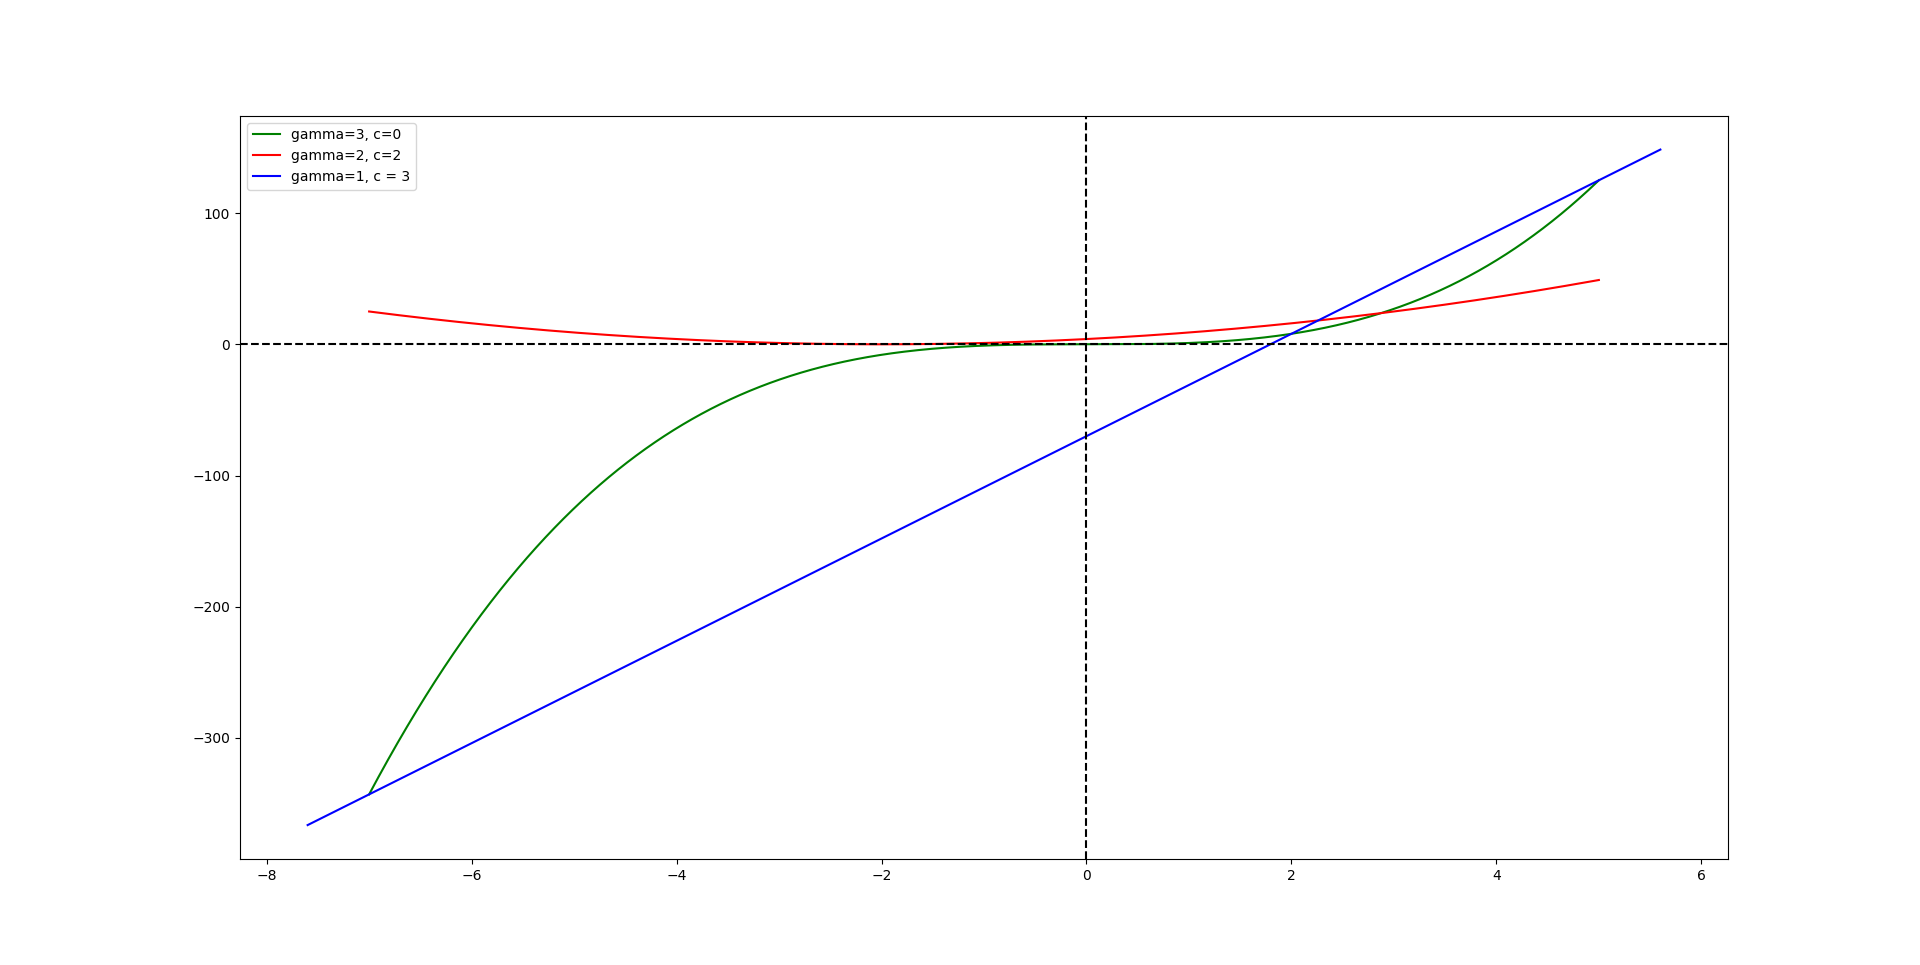
\includegraphics[width=.45\textwidth]{images/samples/polys}
					}
					{
						\caption*{Kernels Polynomiaux avec différentes valeurs de $\gamma$ et $c$.}\label{fig::polys}
					}
				\end{subfloatrow}
			}
			{
				\caption*{}
			}
			\ffigbox[\FBwidth]
			{
				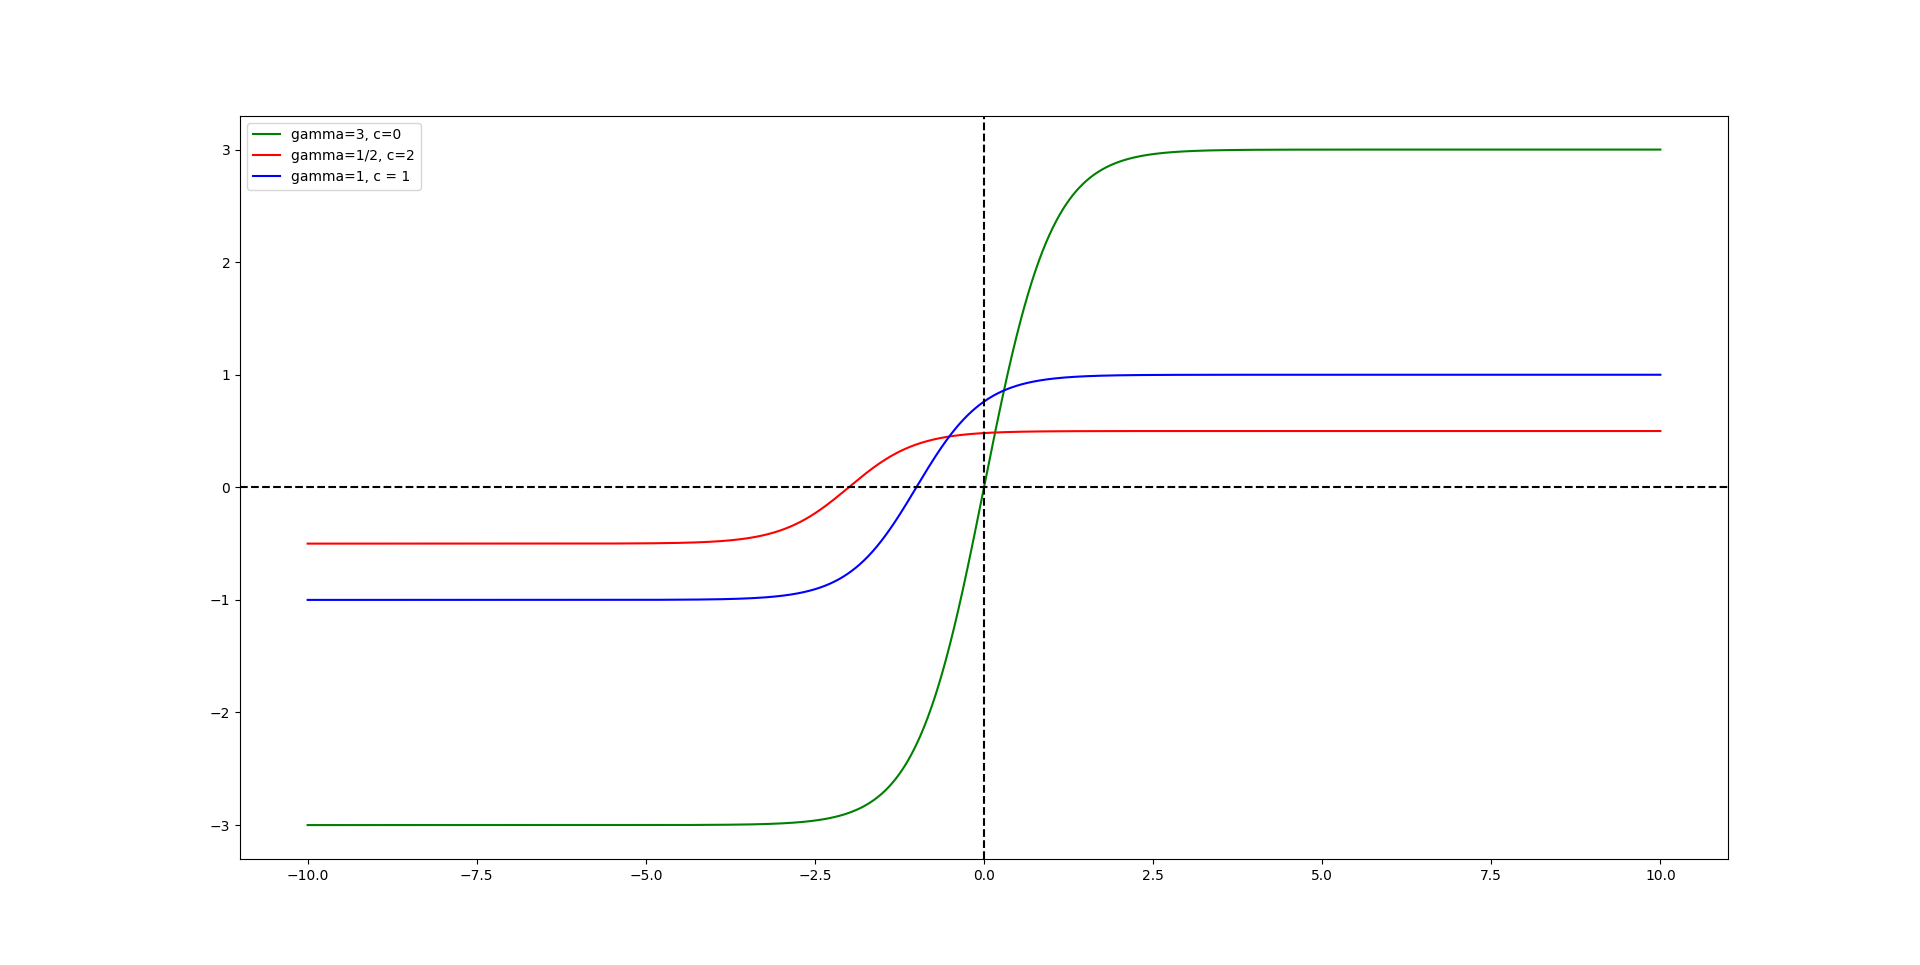
\includegraphics[width=.5\textwidth]{images/samples/tanhs}
			}
			{
				\caption*{Kernels Sigmoids avec différentes valeurs de $\gamma$ et $c$.}\label{fig::tanhs}
			}
		\end{figure}
	\end{frame}

	\section[feature selection]{Sélection d'attributs}
	\subsection[motivation]{Motivation}
	\begin{frame}{Pourquoi sélectionner les attributs?}
		Les espaces de très grande dimension ne ressemblent pas au plan $\mathbb{R}^2$ ou au volume  $\mathbb{R}^3$:
		\begin{itemize}
			\item <1-> Les calculs durent plus de temps,
			\item <2-> Il y a moins de volume à l'intérieur; si on compare le volume contenu dans une sphère et le volume de l'hypercube circonscrit:
			$$\frac{V(\mathbb{B}_{2}(r))}{V(\mathbb{B}_{\infty}(r))}\xrightarrow[d \to \infty]{} 0$$
			\item <3-> La distance Euclidienne n'a plus de sens en très grande dimension $\longrightarrow$ avec moins d'attributs, on peut avoir de meilleurs résultas~\cite{Domingos:2012:FUT:2347736.2347755}.
		\end{itemize}
	\end{frame}

	\begin{frame}{Comment sélectionner les attributs?}
		Encore un fois, sans connaissance préalable, la sélection d'attributs est insoluble vu le nombre exponentiel de possibilité $\sum_{k=0,\dots,n} \begin{pmatrix}
		n\\
		k
		\end{pmatrix} = 2^n$.

		On distingue donc trois types d'approche:
		\begin{enumerate}
			\item<1-> approche par filtre: on choisit les attributs en amont en s'appuyant sur un critère,
			\item<2-> approche intégrée: on sélectionne les attributs en reposant sur les caractéristiques du classifieur,
			\item<3-> approche symbiotique: on sélectionne les attributs les plus performants en aval.
		\end{enumerate}
	\end{frame}

	\subsection[filter approach]{Approche par filtre}
	\begin{frame}{Approche par filtre}
		\begin{itemize}
			\item  Corrélation: un bon sous-ensemble contient des attributs peu corrélés entre eux $\longrightarrow$ on élimine les variables redondantes;
			\item  Relief: évaluation d'un attribut en fonction de sa capacité à discriminer des points proches.
		\end{itemize}
	\end{frame}

	\subsection[integrated approach]{Approche intégrée}
	\begin{frame}{Approche intégrée: cas du SVM-RFE}
		On repose par exemple sur les poids du SVM --- i.e.  $ \textbf{w}$:
		\begin{enumerate}
			\item<1-> On entraine le SVM $\longrightarrow$ on obtient le $\textbf{w}$.
			\item<2-> On choisit l'attribut $i$ avec le plus faible poids:
			$$ i \leftarrow \arg \min_{k=1,\dots,d}{\vert\vert w_k\vert\vert}$$
			\item<3-> On élimine l'attribut $i$.
		\end{enumerate}
		\only<4->{
			On procède donc par récurrence jusqu'au nombre d'attributs cherché~\cite{Guyon2002}.
		}
	\end{frame}

	\subsection[symbiotic approach]{Approche symbiotique}
	\begin{frame}{SFS}
		Sélection ascendante (SFS\@: Sequential Forward Selection).
		\begin{enumerate}
		\item<1-> On sélectionne le meilleur attribut;
		\item<2-> On lui rajoute l'attribut le plus complémentaire;
		\item<3-> On continue à rajouter les attributs de manière à avoir à l'itération $k$ le meilleur $k$-tuple;
		\item <4-> Le problème est qu'on n'a pas de garantie d'obtenir le meilleur ensemble d'attributs.
		\end{enumerate}
	\end{frame}

	\begin{frame}{SFS}
		\begin{block}{Exemple}
			\begin{center}
				\begin{longtable}{c c c c c}
					\toprule
					attributs sélectionés & $1$ & $2$ & $3$ & $4$\\
					\midrule
					résultat& \boldmath $0.49$ & $0.21$ & $0.19$ &$0.24$\\
					\bottomrule
				\end{longtable}
				\begin{longtable}{c c c c c c c}
					\toprule
					attributs sélectionés & $1,2$ & $1,3$ & $1,4$ & $2,3$ & $2,4$ & $3,4$\\
					\midrule
					résultat & \boldmath$0.59$ & $0.51$ & $0.52$ & $0.45$ & $0.49$ & $0.48$\\
					\bottomrule
				\end{longtable}
				\begin{longtable}{c c c c c c c}
					\toprule
					attribut sélectionés & $1,2,3$ & $1,2,4$ & $1,3,4$ & $2,3,4$\\
					\midrule
					résultat & $0.61$ & $0.67$ & $0.59$ & \boldmath$0.78$\\
					\bottomrule
				\end{longtable}
				\begin{longtable}{c c c c c c c}
				\toprule
				attribut sélectionés & $1,2,3,4$\\
				\midrule
				résultat & \boldmath$0.81$\\
				\bottomrule
			\end{longtable}
			\end{center}
		\end{block}
	\end{frame}

	\begin{frame}{SBE}
		Sélection descendante (SBE\@: Sequential Backward Elimination).
		Cette méthode ressemble à celle d'avant.
		\begin{enumerate}
		\item<1-> On élimine le attribut le moins discriminatif;
		\item<2-> On réitère  de telle sorte qu'à l'itération $k$ on aura éleminé les $k$ pires attributs;
		\item<3-> On continue jusqu'à avoir atteint le nombre d'attributs voulus;
		\item <4-> On rencontre le même problème qu'avant.
		\end{enumerate}
	\end{frame}

	\begin{frame}{Comment résoudre le problème donc?}
		\begin{itemize}
			\item<1-> Combinaison SFS + SBE\@: sélection Plus-L-Moins-R\@:
			\begin{itemize}
				\item Si $L > R$, on commence avec un ensemble vide, on ajoute L attributs puis on en enlève R\@,
				\item Si $L < R$, on commence avec tous les attributs, on enlève R attributs puis on en rajoute L\@;
			\end{itemize}
			\item<2-> On garantit la convergence vers une solution unique:
			\begin{itemize}
				\item On peut vérifier que SFS et SBE ne se contredisent pas.
				\item On peut procéder comme dans l'exemple:
				\begin{block}{Exemple}
					Si SFS veut ajouter un attribut, il vérifie qu'il n'a pas été éliminé par SBE\@. Si oui, il prend le 2$^{\text{ème}}$ meilleur et ainsi de suite.
				\end{block}
			\end{itemize}
		\end{itemize}
	\end{frame}

	\section{Références}
	\begin{frame}[allowframebreaks]{Références}
		\nocite{sklearn_api}
		\nocite{camps2009kernel}
		\nocite{CC01a}
		\bibliographystyle{apalike}
		\bibliography{references.bib}
	\end{frame}

\end{document}
